\documentclass[11pt, a4paper, openright, DIV12, BCOR=1cm]{scrbook}

\usepackage{scrhack} %Hacks around some old packages --> less warnings :-)

% language
\usepackage[american]{babel}
\usepackage[utf8]{inputenc}

% bib
\bibliographystyle{plainurl}

\usepackage{amsmath}
\usepackage{amsfonts}
\usepackage{amsthm}
\usepackage{url}

% I need them :-)
\usepackage[plainpages=false]{hyperref}
\hypersetup {
   pdfauthor={Johannes Wei\ss},
   pdftitle={Diplomarbeit Johannes Wei\ss},
   pdfsubject={Diploma Thesis},
   pdfkeywords={KIT, crypto, diploma thesis, Diplomarbeit, Informatik, computer
   science}
}
\usepackage{listings}
\usepackage{color}
\usepackage{tikz}
\usepackage{graphicx}

% DRAFT WATERMARK
\usepackage{draftwatermark}
\SetWatermarkText{DRAFT}
\SetWatermarkScale{4.0}

% other setup
\setcounter{secnumdepth}{3}
\setcounter{tocdepth}{3}


%
% SPECIAL IMPORTS
%
\usepackage{xparse}
\usepackage{boxedminipage}


%
% GENERAL
%

% environments
\NewDocumentEnvironment{JWboxed}{mm}%
  {\begin{figure}[ht]%
   \small%
   \begin{boxedminipage}{\linewidth}%
  }%
  {\end{boxedminipage}%
   \caption{#1}%
   \label{#2}%
   \end{figure}%
  }

% functionality
\newenvironment{JWfunc}[3]%
{\begin{JWboxed}{#2}{#3}%
 \begin{center}\textbf{{Functionality #1}}\end{center}%
}%
{\end{JWboxed}}

\newenvironment{JWfuncSteps}[0]{\begin{itemize}}{\end{itemize}}

\newcommand{\JWfuncSym}[2]{$\mathcal{F}^\mathrm{#1}_\mathrm{#2}$}

%protocol
\newenvironment{JWprotocol}[3]%
{\begin{JWboxed}{#2}{#3}%
 \begin{center}\textbf{{Protocol #1}}\end{center}%
}%
{\end{JWboxed}}

\newenvironment{JWprotoSteps}[0]{\begin{enumerate}}{\end{enumerate}}

\newcommand{\JWprotoPhase}[1]{\paragraph{#1}}

\newcommand{\JWprotoSym}[2]{$\Pi^\mathrm{#1}_\mathrm{#2}$}

%misc
\newcommand{\JWbinary}[1]{\texttt{#1}}
\newcommand{\JWtodo}[1]{\fbox{TODO: #1}}
\newcommand{\JWmsgTT}[2]{(\texttt{#1}, \texttt{#2})}
\newcommand{\JWmsgT}[1]{(\texttt{#1})}
\newcommand{\JWmsgTP}[2]{(\texttt{#1}, #2)}
\newcommand{\JWpath}[1]{\texttt{#1}}

\DeclareDocumentCommand\JWdef{mmg}{%
  {\label{def:#2}\emph{#1\IfNoValueF{#3}{#3}}%
  } (#2%
  \IfNoValueF{#3}{#3}%
  )%
}

\newenvironment{JWtodoBox}[0]%
  {\begin{boxedminipage}{\linewidth}TODO:\par}{\end{boxedminipage}}

%chapters
\makeatletter
\newcommand{\JWlone}{\@ifstar
  \JWloneNoTOC%
  \JWloneTOC%
}
\newcommand{\JWltwo}{\@ifstar
  \JWltwoNoTOC%
  \JWltwoTOC%
}
\newcommand{\JWlthree}{\@ifstar
  \JWlthreeNoTOC%
  \JWlthreeTOC%
}
\newcommand{\JWlfour}{\@ifstar
  \JWlfourNoTOC%
  \JWlfourTOC%
}
\newcommand{\JWlfive}{\@ifstar
  \JWlfiveNoTOC%
  \JWlfiveTOC%
}
\newcommand{\JWlsix}{\@ifstar
  \JWlsixNoTOC%
  \JWlsixTOC%
}

\newcommand{\JWloneTOC}[1]{\chapter{#1}}
\newcommand{\JWloneNoTOC}[1]{\chapter*{#1}}
\newcommand{\JWltwoTOC}[1]{\section{#1}}
\newcommand{\JWltwoNoTOC}[1]{\section*{#1}}
\newcommand{\JWlthreeTOC}[1]{\subsection{#1}}
\newcommand{\JWlthreeNoTOC}[1]{\subsection*{#1}}
\newcommand{\JWlfourTOC}[1]{\subsubsection{#1}}
\newcommand{\JWlfourNoTOC}[1]{\subsubsection*{#1}}
\newcommand{\JWlfiveTOC}[1]{\paragraph{#1}}
\newcommand{\JWlfiveNoTOC}[1]{\paragraph*{#1}}
\newcommand{\JWlsixTOC}[1]{\subparagraph{#1}}
\newcommand{\JWlsixNoTOC}[1]{\subparagraph*{#1}}

%links and names
\newcommand{\JWnamedlink}[2]{\href{#1}{#2}}
\newcommand{\JWurl}[1]{\href{#1}{#1}}

%code/commands
\newcommand{\JWcode}[1]{\texttt{#1}}
\newcommand{\JWcmd}[1]{\texttt{\$ #1}}
\newcommand{\JWhsExt}[1]{\texttt{#1}}


%lemmata/theorems
\newtheorem{thm}{Theorem}
\newtheorem{lem}[thm]{Lemma}


%
% SPECIALIZED SHORTCUTS
%
\newcommand{\JWprotoSymOPE}[0]{\JWprotoSym{}{OPE}}
\newcommand{\JWfuncSymOPE}[0]{\JWfuncSym{(k, n)}{OPE}}
\newcommand{\JWfuncSymOPEnp}[0]{\JWfuncSym{}{OPE}}
\newcommand{\JWfuncSymOAFE}[0]{\JWfuncSym{seq-ot}{OAFE}}
\newcommand{\JWfieldGeneral}[0]{\mathbb{F}_{2^k}}
\newcommand{\JWadv}[0]{$\mathcal{A}$}
\newcommand{\JWpOne}[0]{Goliath}
\newcommand{\JWpTwo}[0]{David}
\newcommand{\JWtoken}[0]{Token}
\newcommand{\JWnegl}[0]{\text{*) Except for a negligible probability.}}
\newcommand{\JWtitle}[0]{Efficient Secure Function Evaluation using Garbled %
Arithmetic Circuits and Untrusted Tamper--Proof Hardware}
\newcommand{\entspricht}{\stackrel{\scriptscriptstyle\wedge}{=}}

%tools ans versions
\newcommand{\JWThaskell}[0]{Haskell}
\newcommand{\JWTghc}[0]{GHC}
\newcommand{\JWTXghc}[0]{Glasgow Haskell Compiler}
\newcommand{\JWTLhaskell}[0]{\JWnamedlink{http://haskell.org}{\JWThaskell}}
\newcommand{\JWTLhaddock}[0]{\JWnamedlink{http://www.haskell.org/haddock/}%
                            {Haddock}}
\newcommand{\JWTLcabal}[0]{\JWnamedlink{http://www.haskell.org/cabal/}%
                            {Cabal}}
\newcommand{\JWTXLghc}[0]{\JWnamedlink{http://www.haskell.org/ghc/}{\JWTXghc}}
\newcommand{\JWTVghc}{7.6.1}
\newcommand{\JWTntl}[0]{NTL}
\newcommand{\JWTLntl}[0]{\JWnamedlink{http://www.shoup.net/ntl/}{\JWTntl}}
\newcommand{\JWTcpp}[0]{C++}
\newcommand{\JWTc}[0]{C}
\newcommand{\JWTgit}[0]{git}
\newcommand{\JWTquickcheck}[0]{QuickCheck}
\newcommand{\JWTLhunit}[0]{\JWnamedlink{http://hunit.sourceforge.net/}{HUnit}}
\newcommand{\JWTLmonadcryptorandom}[0]%
  {\JWnamedlink{http://hackage.haskell.org/package/monadcryptorandom}%
  {\texttt{monadcryptorandom}}}
\newcommand{\JWTLhaskellForMaths}[0]%
  {\JWnamedlink{http://hackage.haskell.org/package/HaskellForMaths}%
  {\texttt{HaskellForMaths}}}
\newcommand{\JWTLdrbg}[0]%
  {\JWnamedlink{http://hackage.haskell.org/package/DRBG}{\texttt{DRBG}}}
\newcommand{\JWTXprotobuf}{Google\TTra{} Protocol Buffers}
\newcommand{\JWTprotobuf}{Protocol Buffers}
\newcommand{\JWTXLprotobuf}[0]%
  {\JWnamedlink{http://code.google.com/apis/protocolbuffers/}{\JWTXprotobuf{}}}
\newcommand{\JWTLhackage}[0]%
  {\JWnamedlink{http://hackage.haskell.org/packages/hackage.html}{HackageDB}}


%binaries
\newcommand{\JWBpOne}[0]{\JWbinary{\JWpOne{}}}
\newcommand{\JWBpTwo}[0]{\JWbinary{\JWpTwo{}}}
\newcommand{\JWBtoken}[0]{\JWbinary{\JWtoken{}}}

%misc
\newcommand{\JWport}[1]{\texttt{#1}}
\def\TReg{\textsuperscript{\textregistered}}
\def\TCop{\textsuperscript{\textcopyright}}
\def\TTra{\textsuperscript{\texttrademark}}


\title{Efficient Secure Function Evaluation using Garbled Arithmetic Circuits
and Untrusted Tamper--Proof Hardware}

\author{Johannes Weiß}

\begin{document}

\selectlanguage{american}

\pagenumbering{Roman}

\pagenumbering{Roman}

\thispagestyle{empty}

\begin{picture}(0,0)(85,770)

\includegraphics[width=\paperwidth]{images/KIT_Deckblatt}
\end{picture}


\begin{center}
\hbox{}
\vfill
{ \sffamily
{\huge\bfseries \JWtitle{} \par}
\vskip 1.8cm
Diplomarbeit\\
\vskip 1cm

{\large\bfseries Johannes Weiß\\}
\vskip 1.2cm
Institut für Kryptographie und Sicherheit\\
Europäisches Institut für Systemsicherheit\\
Fakultät für Informatik\\
Karlsruher Institut für Technologie\\
\vskip 3cm
\begin{tabular}{p{5.5cm}l}
Betreuender Professor:&{\sffamily Prof.\ Dr.\ rer.\ nat.\ Jörn Müller--Quade} \\
Betreuender Mitarbeiter: & Dipl.-Inform. Daniel Kraschewski
\end{tabular}
\vskip 3cm
Bearbeitungszeit:\qquad 1.\ Juli 2012 -- 31.\ Dezember 2012
}
\end{center}
\vfill

\cleardoublepage{}

\thispagestyle{empty}

\vspace*{\fill}

\noindent{}{\Large Eigenst\"andigkeitserkl\"arung}

\bigskip{}

\noindent{}Hiermit versichere ich, dass ich die Arbeit selbstst\"andig verfasst
habe und keine anderen als die angegebenen Quellen und Hilfsmittel benutzt habe,
die w\"ortlich oder inhaltlich \"ubernommenen Stellen als solche kenntlich
gemacht habe und die Satzung des Karlsruher Instituts f\"ur Technologie zur
Sicherung guter wissenschaftlicher Praxis in der g\"ultigen Fassung beachtet
habe.

\bigskip{}

Karlsruhe, den 18.\ Dezember 2012

\bigskip{}

\bigskip{}

\bigskip{}

Johannes Wei\ss

\vspace*{\fill}

\cleardoublepage

\thispagestyle{empty}

\vspace*{\fill}
\begin{center}
{\Large \JWtitle{}} \\
Johannes Wei\ss{} $<$diplomarbeit@johannesweiss.eu$>$
\end{center}
\vspace*{\fill}

\newpage
\thispagestyle{empty}

\null
\vfill
\hfill Typeset using \LaTeX{} on \today{}, \currenttime{}.
\input{res/git-state.tex}


\frontmatter
\tableofcontents

\mainmatter

\cleardoublepage

\JWlone{Introduction}
\label{sec:introduction}

A \JWdef{Secure Multi--Party Computation}{MPC} or \JWdef{Secure Function
Evaluation}{SFE} is the joint calculation of an arbitrary function $f$ with
private inputs from a set of mutually distrusting parties. If the size of the
set of parties for an MPC is two, the computation is also called a two--party
computation. The area of research of secure multi--party computations was
founded by Yao \cite{yao82}. His famous \emph{Millionaires' Problem} discusses
two millionaires, who are interested in knowing which of them is richer without
revealing the actual values of their wealth. The problem is evaluating the
function $f(a, b) = a \geq b$, where the first millionaire inputs the value of
his wealth as $a$ and the second inputs $b$. The result of the evaluation is
either \textit{false} if the second millionaire is richer or \textit{true}
meaning the opposite. From the result and the own input, neither party is able
to calculate the wealth of the other millionaire. Another example for
real--world multi--party computations are democratic elections. The eligible
voters input their private vote and the result of the calculation is the
percentage breakdown.

\JWdefn{Oblivious Polynomial Evaluation}{OPE} \cite{naor99,naor06} is a special
case of SFE\@. In contrast to arbitrary functions that are known by the involved
parties, OPE only allows the first party to privately submit a polynomial $p$
and another party to evaluate the polynomial at one node $x$. The second party
obtains the result $p(x)$ but not the polynomial, the first party learns
nothing. A secure and efficient OPE protocol is a useful and interesting
primitive because many other cryptographic problems can be based on OPE, for
example the share generation for \emph{Shamir's Secret Sharing} \cite{shamir79}.

\JWdefn{Oblivious Affine Function Evaluation}{OAFE} \cite{davidgoliath} is a
primitive that allows to obliviously evaluate affine functions. The David \&
Goliath protocol \cite{davidgoliath} presents a secure and efficient OAFE
implementation based on only one stateful tamper--proof hardware token. Based on
OAFE, this thesis works out the novel result of OPE in linear time which
is asymptotically as fast as usual polynomial evaluation. Alongside the
theoretical methodology, this thesis features an efficient, secure, and working
implementation of the proposed protocol. The presented approaches are also
suitable for general SFE (including \emph{Square \& Multiply} \cite{knuth81}),
however the security is only proved for OPE\@. The security of the protocol
against passive and active adversaries is in\-for\-ma\-tion--the\-o\-ret\-ically
proved in the \JWdefn{Universal Composability}{UC} framework \cite{canetti05}.


%
% RELATED WORK
%
\JWltwo{Related Work}
\label{sec:related-work}

The notion of \emph{universal composability} in the UC framework by Canetti
\cite{canetti05} places strict demands on the security of cryptographic
protocols. Proofs in the UC framework have to show that any environment is
unable to distinguish between an ideal functionality and the implemented
protocol, even when malicious adversaries misuse the protocol in some
unpredictable way. The benefit of the strict requirements of this notion is that
UC--secure protocols can be composed and ran concurrently while still staying
safe without the necessity of additional security proofs. This thesis uses
universal composability as the notion of security.

Yao defined the problem of multi--party computations and his \JWdefn{Garbled
Circuit}{GC} approach \cite{yao86} describes encrypted evaluation of (boolean)
circuits. But despite the versatility of Yao's garbled circuits, the approach is
not suitable for arithmetic functions on large fields. Because the GC approach
requires embedded truth tables in every gate, an adoption to larger finite
fields would have the consequence of a quadratic blowup of every truth table in
every gate (cf.\ \cite{naor99privacy}). This thesis solves these problem
efficiently for arbitrary polynomials.

Besides the GC approach, this thesis is also related to \emph{Efficient
Multi-Party Computation Over Rings} by Cramer et al.~\cite{cramer03}. The
difference is that Cramer's approach is based on the simulation of formulas by
bounded--width programs by Cleve \cite{cleve91} which does not support
\emph{Square \& Multiply} \cite{knuth81} and the complexity is polynomial (with
a low degree) in the number of arithmetic operations performed. The writings of
Naor et al.~\cite{naor99,naor06} also describe OPE but have polynomial
complexity and based on \JWdefn{Oblivious Transfer}{OT} \cite{rabin81}.

\emph{How to Garble Arithmetic Circuits} by Applebaum et al.~\cite{gac2012}
describes the garbled evaluation of arithmetic circuits.  Many ideas used in
this thesis are inspired by Applebaum et al. The difference between
Applebaum's paper and this thesis, is that the former relies on computational
assumptions to be secure. In contrast, this thesis does not rely on
computational assumptions and proves the methodology to be
information--theoretically secure. This thesis adapts some of Applebaum's ideas
to work with \JWdefn{Oblivious Affine Function Evaluation}{OAFE}
\cite{davidgoliath}.

%
% ACKNOWLEDGMENTS
%
\JWltwo{Acknowledgments}

I wish to thank my advisor Daniel Kraschewski who supported me throughout the
research and writing of this thesis. He donated a large amount of his limited
time for discussions and explorations crucial for my thesis and allowed this
thesis to be my own work but steered me in the right direction when needed.  I
am also thankful for his patience introducing me to this exciting topic.


%
% Outline
%
\JWltwo{Outline}

This thesis starts by introducing the reader to the general methodology, which
is discussed in depth thereafter (Chapter \ref{sec:methods}). Next, the security
of the methodology is analyzed and proved in the UC framework (Chapter
\ref{sec:security}). Since this thesis also implements the proposed protocol,
the implementation is covered in Chapter \ref{sec:implementation}. An evaluation
of both, the methodology and the implementation (Chapter \ref{sec:evaluation})
followed by the conclusion (Chapter \ref{sec:conclusion}) rounds out this
thesis.  And since a large amount of the time taken for this thesis was affected
by researching, a brief tour of the discontinued approaches is given to the
reader (Chapter \ref{sec:discontinued}).

% vim: set spell spelllang=en_us fileencoding=utf8 formatoptions=tcroql : %


\JWlone{Methods}
\label{sec:methods}

\begin{JWtodoBox}

  Top--down Beschreibung was getan werden soll:

  \begin{itemize}

    \item Halbtechnisch

    \item Von einem Informatiker zu verstehen

    \item Gewisse Art von Motivation von dem dann folgenden sehr detaillierten
      bottom--up approach

  \end{itemize}

\end{JWtodoBox}

This chapter describes how arbitrary arithmetic functions can be expressed in
terms of affine expressions. This is the most important part of this thesis
because it is the key part of evaluating arbitrary arithmetic expressions
using OAFEs \cite{davidgoliath}.


%
% DEFINITIONS
%
\JWltwo{Definitions}
\label{sec:rae-definitions}

This chapter defines important entities that are used to define the more complex
entities in the following chapters.

% Field K
\JWlthree*{Field $K$}
\label{sec:field}

\label{def:field} Throughout this thesis, $K$ represents an arbitrary large
finite field, such as $\mathbb{F}_{2^{256}}$.

\JWtodo{Irreduzibled Polynom hinschreiben}


% OAFEs
\JWlthree*{OAFEs}

In this thesis the \JWdef{Oblivious Affine Function Evaluation}{OAFE}{s} are
essentially one \emph{Sequential one--time OAFE} as defined by Döttling,
Kraschewski and Müller-Quade \cite{davidgoliath}. The OAFEs can be used to
obliviously evaluate affine functions $f_i$. The collectivity of all OAFEs (as
defined in this thesis) maps to exactly one tamper--proof hardware token
realizing one \emph{Sequential one--time OAFE} \cite{davidgoliath}:

\begin{align*}
  f_i(x_i) = &
  a_ix_i + b_i \\
%
  = &
\begin{pmatrix}a_{i,1}\\a_{i,2}\\a_{i,3}\\\vdots\end{pmatrix}x_i +
\begin{pmatrix}b_{i,1}\\b_{i,2}\\b_{i,3}\\\vdots\end{pmatrix}
\end{align*}

\noindent{}Obviously, every function $f_i$ can only be evaluated only once and
the functions $f_i$ have to be evaluated in order: $f_1$ being the first, $f_2$
the second and so forth.

In this thesis usually the term OAFEs is used to denote the fact that there are
multiple affine functions ($f_i$) that can be evaluated obliviously. The term
OAFE configuration is used to denote the vectors $a_i$ and $b_i$. One OAFE
configuration is the same as the collectivity of the $(a_i, b_i, i)$ triples as
used in the original definition \cite{davidgoliath}.


%
% DUAL RANDOMIZED AFFINE VALUES
%
\JWltwo{Dual Randomized Affine Values}
\label{sec:drav}

\JWdef{Dual Randomized Affine Value}{DRAV}{s} are encrypted, signed values
representing a scalar value of the field $K$. Each DRAV is encrypted by a pair
of \emph{dual keys}. The first dual key, the \emph{static key}, remains the same
in the whole DRAC (see chapter \ref{def:DRAC}) generation procedure and is
usually denoted as $(\alpha_l, \alpha_r)$. The second dual key, the
\emph{dynamic key} is a short--lived key, usually represented as $(\beta,
\beta')$. Two DRAVs only share the same dynamic key by hazard but always share
the same static key. Encoding a regular value $v \in K$ as a DRAV
$\widetilde{v} \in \mathcal{V}_K$ is straightforward, most of the time the
universal encoding function $E(v)$ is used to describe DRAV encoding. For the
sake of simplicity $E(v)$ is already parametrized by the static dual key
$(\alpha_l, \alpha_r)$ and is able to generate a new dynamic dual key $(\beta,
\beta')$ uniformly at random. $D(\widetilde{v})$ is assumed to know the correct
decryption keys.

\begin{align*}
  \widetilde{v} = E(v) = (\widetilde{v_l}, \widetilde{v_r}) =
    (\alpha_l \cdot v + \beta, \alpha_r \cdot v + \beta')
\end{align*}

\noindent{}So, if the keys are uniformly at random, the two components of the
tuple $\widetilde{v}$ are uniformly at random, too. Decoding is (most of the
time using the universal decoding function $D(\widetilde{v})$):

\begin{align*}
  v = D(\widetilde{v}) =
  \left\{
    \begin{array}{l l}
      \frac{\widetilde{v_l} - \beta}{\alpha_l} & \quad
      \text{if}~\frac{\widetilde{v_l} - \beta}{\alpha_l} =
      \frac{\widetilde{v_r} - \beta'}{\alpha_r}\\
      \bot & \quad \text{otherwise ($\widetilde{v}$ is non--well--formed)}\\
    \end{array}\right.
\end{align*}


% WELL-FORMED DRAVs
\JWlthree{Well--Formed DRAVs}

A DRAV $\widetilde{v}$ is well--formed iff $D(\widetilde{v}) \neq \bot$.
Therefore, if $D(\widetilde{\chi}) = \bot$, $\chi$ is non--well-formed.


% DIRECT DRAV ARITHMETIC
\JWlthree{Direct DRAV Arithmetic}
\label{sec:direct-DRAV-arithmetic}

Direct DRAV arithmetic only supports addition ($+$) of two DRAVs. Indirect DRAV
arithmetic has to be used for other operations. The advantage of direct DRAV
arithmetic is that it can be performed without the knowledge of a DRAV's
encryption keys.

\paragraph{Addition of Well--Formed DRAVs:} Two DRAVs $\widetilde{x} =
(\widetilde{x_l}, \widetilde{x_r})$ and $\widetilde{y} = (\widetilde{y_l},
\widetilde{y_r})$ can be added componentwise to $\widetilde{z} =
\left(\widetilde{x_1} + \widetilde{y_1}, \widetilde{x_2} +
\widetilde{y_2}\right)$. The encryption keys for $\widetilde{z}$ will be
$(\alpha_l, \alpha_r)$ and $(\beta_1 + \beta_3, \beta_2 + \beta_4)$ assuming
$\widetilde{x}$ was encrypted with $(\alpha_l, \alpha_r)$ and $(\beta_1,
\beta_2)$ and $y$ was encrypted with $(\alpha_l, \alpha_r)$ and $(\beta_3,
\beta_4)$.

\subparagraph{Proof:} From ($\widetilde{x} = \left(\alpha_l \cdot x + \beta_1,
\alpha_r \cdot x + \beta_2\right)$, $\widetilde{y} = \left(\alpha_l \cdot x +
\beta_3, \alpha_r \cdot x + \beta_4\right)$) it's obvious that: $\widetilde{z} =
\left(\alpha_l \cdot (x+y) + (\beta_1 + \beta_3), \alpha_r \cdot (x+y) +
(\beta_2 + \beta_4)\right)$ and $\widetilde{z}$ is well--formed.

\paragraph{Addition of Non--Well--Formed DRAVs:} It's of particular interest the
following property holds: $\forall \widetilde{x}: \widetilde{x} + \bot = \bot
+ \widetilde{x} = \bot$. Let $\widetilde{\chi}$ be a non--well--formed DRAV,
so: $\widetilde{\chi} = (\alpha_l \cdot \chi + \beta_3 + \Delta_l, \alpha_r
\cdot \chi + \beta_4 + \Delta_r)$. The component--wise addition
$\widetilde{\nu}$ of $\widetilde{\chi}$ to any well--formed $\widetilde{x} =
(\alpha_l \cdot x + \beta_1, \alpha_r \cdot x + \beta_2)$ is $\widetilde{\nu} =
(\alpha_l \cdot (x+\chi) + (\beta_1+\beta_3) + \Delta_l, \alpha_r \cdot (x+\chi)
+ (\beta_2+\beta_4) + \Delta_r)$. Using the universal decoding function $D$, the
value of $\chi$ is $\chi = D(\widetilde{\chi}) = (x + \chi +
\frac{\Delta_l}{\alpha_l}, x + \chi + \frac{\Delta_r}{\alpha_r})$. So: $\forall
(\Delta_r, \Delta_l) \in K \setminus \{(0, 0)\} \wedge \frac{\Delta_l}{\alpha_l}
\neq \frac{\Delta_r}{\alpha_r}: D(\widetilde{\chi}) = \bot$. Since the
encryption keys are not known to an attacker, $\frac{\Delta_l}{\alpha_l} \neq 0
\wedge \frac{\Delta_r}{\alpha_r}$ hold except for a negligible probability if
$\Delta_r \neq 0 \vee \Delta_r \neq 0$ and that's the property for being forged
(non--well--formed) which was the assumption. Trivially $\bot + \bot = \bot$ by
a similar argument.


% INDIRECT DRAV ARITHMETIC
\JWlthree{Indirect DRAV Arithmetic}
\label{sec:indirect-DRAV-arithmetic}

Indirect DRAV arithmetic assumes the universal encoding and decoding functions
$E(v)$ and $D(\widetilde{v})$ and therefore the knowledge of the encryption
keys. Another possibility is to map indirect DRAV arithmetic to OAFE calls that
are set up by a party that knows the encryption keys.

Indirect DRAV arithmetic is straightforward but can only be performed by a party
in possession of the encryption keys. For any operator $\odot$, $\widetilde{a}
\odot \widetilde{b} = E(D(\widetilde{a}) \odot D(\widetilde{b}))$. Obviously
it's important that $\forall x: \bot \odot x = x \odot \bot = \bot$. $\bot$ can
be represented as a DRAV as a tuple that is made up of two values uniform at
random.


% FINAL DRAV DECODING
\JWlthree{Final DRAV Decoding}
\label{sec:drav-final-decoding}

Finally decoding a DRAV can be trivially done using the universal decoding
function $D(\widetilde{v})$. But $D$ is only available to a party that is in
possession of the encryption keys.

Additionally a DRAV can also be finally decoded only one additional OAFE call.
The following procedure will decode a DRAV to a final scalar value although
$D$ is a partial function. To enable a second party---that is not in possession
of the encryption keys---to decode a DRAV $\widetilde{v} = (\widetilde{v_1},
\widetilde{v_2})$, the first party---in possession of the keys---needs to set up
a special OAFE, called the \emph{final OAFE} below.

The second party's input to the final OAFE is $\widehat{v} = \widetilde{v_1} +
\widetilde{v_2}$, the addition of both components of the DRAV to decode.  The
final OAFE was set up by the first party as follows: Assuming $\widetilde{v}$ is
encrypted by $(\alpha_l, \alpha_r)$ and $(\beta_1, \beta_2)$ the first party
knows $\widehat{v}$ has to be encrypted using $(\alpha_l + \alpha_r)$ and
$(\beta_1 + \beta_2)$.  Given this knowledge the final OAFE setup is
$\frac{1}{\alpha_l + \alpha_r} \cdot \widehat{v} - \frac{\beta_1 +
\beta_2}{\alpha_l + \alpha_r}$.

Again, it's important that an attacker is getting caught when trying to forge a
DRAV ($D(\widetilde{v}) = \bot$ if $\widetilde{v}$ has been forged, $\bot$ is
mapped to uniform randomness in this process since an OAFE has no
$\bot$--value). If the attacker cheated somewhere in the process and forged one
of the DRAV tuples $\widetilde{x} = (\widetilde{x_1}, \widetilde{x_2})$ to
$\widetilde{x'} = (\widetilde{x_1} + \Delta_1, \widetilde{x_2} + \Delta_2)$, the
DRAV $\widetilde{x'}$ becomes---except for a negligible
probability---non--well--formed (see section \ref{sec:drav}). The result is that
the decoded result will become uniform randomness (assuming $\widetilde{x}$ is
forged to $\widetilde{x'_1} = \widetilde{x_1} + \Delta_1$ and $\widetilde{x'_2}
= \widetilde{x_2} + \Delta_2$):

\begin{align*}
  \widehat{x'} = & \widetilde{x'_1} + \widetilde{x'_2} = \widetilde{x_1} +
  \Delta_1 + \widetilde{x_2} + \Delta_2 \\
  %
  \Rightarrow x' = & \frac{1}{\alpha_l + \alpha_v} \cdot \widehat{x'} -
  \frac{\beta_{x_1} +
  \beta_{x_2}}{\alpha_l + \alpha_v} \\
  %
  \Leftrightarrow x' = & \frac{\widetilde{x_1} + \Delta_1 +
  \widetilde{x_2} + \Delta_2}{\alpha_l + \alpha_v} -
  \frac{\beta_{x_1} +\beta_{x_2}}{\alpha_l + \alpha_v}\\
  %
  \Leftrightarrow x' = & \frac{(\alpha_l x + \beta_{x_1}) + \Delta_1 +
  (\alpha_v x + \beta_{x_2}) + \Delta_2}{\alpha_v + \alpha_l} -
  \frac{\beta_{x_1} +\beta_{x_2}}{\alpha_l + \alpha_v} \\
  %
  \Leftrightarrow x' = & \frac{(\alpha_l+\alpha_v)x + (\beta_{x_1}+\beta_{x_2} +
  \Delta_1+\Delta_2)}{\alpha_l+\alpha_v} -
  \frac{\beta_{x_1} +\beta_{x_2}}{\alpha_l + \alpha_v} \\
  %
  \Leftrightarrow x' = & x + \frac{\beta_{x_1}+\beta_{x_2}}{\alpha_l+\alpha_v}
  + \frac{\Delta_1 + \Delta_2}{\alpha_l + \alpha_v} -
  \frac{\beta_{x_1}+\beta_{x_2}}{\alpha_l + \alpha_v} \\
  %
  \Leftrightarrow x' = & x + \frac{\Delta_1 + \Delta_2}{\alpha_l + \alpha_v}\\
\end{align*}

Because an attacker is not in possession of the static encryption keys
$\alpha_l$ and $\alpha_r$, it cannot control the value of $\frac{\Delta_1 +
\Delta_2}{\alpha_l + \alpha_r}$. Since $\alpha_l$ and $\alpha_r$ are chosen
uniform at random, the result $x'$ becomes uniform at random, too.


%
% DUAL RANDOMIZED AFFINE ENCODING
%
\JWltwo{Dual Randomized Affine Encoding}
\label{sec:drae}

\JWdef{Dual Randomized Affine Encoding}{DRAE}{s} are affine representations of
parts of arithmetic circuits that fulfill several properties:

\begin{enumerate}

  \item \label{prop:drae-encrypted} DRAEs are encrypted: Without the encryption
    keys, they don't reveal any information.

  \item \label{prop:drae-signed} DRAEs are signed: If someone tries to forge a
    DRAE, it will become non--well--formed and operations with that DRAE result
    in non--well--formed DRAEs.

  \item \label{prop:drae-oafe} DRAEs can be securely evaluated using OAFEs.

  \item \label{prop:drae-not-enough} DRAEs can not express arbitrary arithmetic
    circuits alone.

\end{enumerate}

\noindent{}A DRAE can be eventually evaluated to a final value, that is a DRAV
(see chapter \ref{def:DRAV}). Informally, a DRAE is composed of two finite
multi--sets. The first multi--set, called the \emph{multiplicative terms}
contains tuples of computations. The second multi--set, called the
\emph{additive terms} contains computations that can be evaluated to DRAVs. The
component--wise multiplication of each of the computation tuples (from the
multiplicative terms) yields DRAVs, too. The addition of all the DRAVs obtained
from the additive terms and all the DRAVs obtained from the multiplicative terms
leads to a DRAV that is the evaluation of this DRAE.

More formally, a DRAE can be described as follows where $\mathcal{E}$ represents
the DRAEs, $\mathcal{C}$ the computations and $\mathcal{V}_\mathcal{C}$ the
computations that lead to DRAVs.

\begin{align}
%
  &\text{The static keys } \alpha_l, \alpha_r \in K \setminus \{0\} \nonumber\\
%
  &\text{The dynamic keys } \beta, \beta' \in K \nonumber\\
%
  &s, x, x', i \in K \nonumber\\
%
  \mathcal{C} = & \{ c(x) = s \cdot x + i \} \nonumber\\
%
  \mathcal{V}_\mathcal{C} = & \{ (\alpha_l \cdot f(x) + \beta,
                      \alpha_r \cdot f'(x') + \beta' )
                    \mid f, f' \in \mathcal{C} \} \nonumber\\
%
  \label{rel:DRAE}
  \mathcal{E}_\mathcal{C} = & \{ (M, A) \mid
      M \subseteq \mathcal{V}_\mathcal{C} \times
      \mathcal{V}_\mathcal{C}, A \subseteq, \mathcal{V}_\mathcal{C};
  A, M~\text{finite multi--sets} \}
%
\end{align}

Pre--evaluating a DRAE to DRAVs can be done by evaluating the OAFEs set up by
the party in possession of the encryption keys. Obviously none of the
computations $c \in \mathcal{C}$ becomes visible by the party not in possession
of the keys. The latter party will only learn exactly one evaluation $c(x)$ for
each variable $x$. This leads to pre--evaluated DRAEs of the form

\begin{align}
  \mathcal{V} = & \{ (v_l, v_r) \mid v_l, v_r \in K \}
  \text{, the DRAVs (chapter \ref{def:DRAV})} \nonumber\\
%
  \label{rel:pre-eval-DRAE}
  \mathcal{E} = & \{ (M, A) \mid
      M \subseteq \mathcal{V} \times \mathcal{V}, A \subseteq, \mathcal{V} \}
      \text{, the pre--evaluated DRAEs}
\end{align}

Evaluating a pre--evaluated DRAE is straightforward: A DRAE $e \in \mathcal{E} =
(M,A)$ can be evaluated to its single resulting DRAV $r \in \mathcal{V}$ as
follows (all additions performed component--wise):

\begin{align*}
M' &= \Bigg\{ m_1 \cdot m_2\ \Bigg|\ \begin{pmatrix}m_1\\m_2\end{pmatrix}
\in M \Bigg\} \\
r & = \sum_{a \in A}a + \sum_{m \in M'}m
\end{align*}


% DRAE ARITHMETIC
\JWlthree{DRAE Arithmetic}

%Direct Addition
\JWlfour{Addition}

Since two DRAVs can directly be added as explained in chapter
\ref{sec:direct-DRAV-arithmetic}, two DRAEs can be added by concatenating the
multiplicative ($M$ in relations \ref{rel:DRAE} and \ref{rel:pre-eval-DRAE}) and
additive ($A$) terms. Notably, although the encryption keys change, this
operation can be performed by any party, in possession of the encryption keys or
not. Obviously, the same argument holds for pre--evaluated DRAEs.


%Indirect Addition
\JWlfour{Indirect Addition via OAFEs}

The indirect addition of $\widetilde{z} = \widetilde{x_1} + \widetilde{x_2}$ is
$\widetilde{z} =
\left( E\left(D(\widetilde{x_1}) + D(\widetilde{y_1})\right),
       E\left(D(\widetilde{x_2}) + D(\widetilde{y_2})\right)
\right)$
(see chapter \ref{sec:indirect-DRAV-arithmetic}).
Since $E(x)$ and $D(x)$ are both linear functions, $E\left(D(\ldots)
+D(\ldots)\right)$ are linear functions, too that can be evaluated using two
OAFE calls.  Obviously the OAFEs have to be configured appropriately by the
party in possession of the encryption keys.


%Multiplication
\JWlfour{Multiplication}

As described in chapter \ref{def:DRAV}, DRAV cannot be multiplied directly.
Therefore DRAVs have to be multiplied indirectly requiring additional OAFE
calls. To maintain the important DRAV and DRAE property that any operation on
bottom ($\bot$) results in bottom, the two components of each DRAV get mixed for
multiplication.

\JWtodo{Warum müssen sie gemixt werden: Das Argument mit gegen
Null prüfen}

\JWtodo{Das Mixen genauer erklären}


\begin{align*}
  E & \in \mathcal{E}; \widetilde{x}, \widetilde{y} \in \mathcal{V};
  r_1, r_2, r_3, r_4, r_5, r_6, r_7, r_8 \in K;
  \alpha_l, \alpha_r \in K \setminus \{0\} \\
  %
  E & = \widetilde{x} \cdot \widetilde{y} \\
  %
  E & = \Bigg(\left\{\left(
            \begin{pmatrix}
              \alpha_l \cdot D(\widetilde{x_1}) - r_1 \\
              \alpha_r \cdot D(\widetilde{x_2}) - r_5
            \end{pmatrix},
            \begin{pmatrix}
              1        \cdot D(\widetilde{y_1}) - r_2 \\
              1        \cdot D(\widetilde{y_2}) - r_6
            \end{pmatrix}
        \right)\right\}, \\
    &   \qquad\bigg\{
        \begin{pmatrix}
            \alpha_lr_2 \cdot D(\widetilde{x_2}) + r_3 \\
            \alpha_rr_6 \cdot D(\widetilde{x_1}) + r_7
          \end{pmatrix} \\
    &  \qquad,
        \ \begin{pmatrix}
            r_1        \cdot D(\widetilde{y_2}) + r_4 \\
            r_5        \cdot D(\widetilde{y_1}) + r_8
          \end{pmatrix}
        \bigg\}\Bigg) \\
\end{align*}

Decoding (see chapter \ref{def:DRAE}) a well--formed $E$ to
$\widetilde{e} \in \mathcal{V}$ leads to:

\begin{align*}
  \widetilde{e} & =
  \begin{pmatrix}
    (\alpha_l \cdot D(\widetilde{x_1})-r_1) \cdot
    (1        \cdot D(\widetilde{y_1})-r_2) \\
    (\alpha_r \cdot D(\widetilde{x_2})-r_5) \cdot
    (1        \cdot D(\widetilde{y_2})-r_6)
  \end{pmatrix}
  +
  \begin{pmatrix}
    \alpha_lr_2 \cdot D(\widetilde{x_2}) + r_3 +
    r_l         \cdot D(\widetilde{y_2}) + r_4 \\
    r_2         \cdot D(\widetilde{x_1}) + r_7 +
    r_5         \cdot D(\widetilde{y_1}) + r_8
  \end{pmatrix} \\
%
  & =
  \begin{pmatrix}
    \alpha_l \cdot D(\widetilde{x_1}) \cdot D(\widetilde{y_1})
    -\alpha_lr_2 \cdot D(\widetilde{x_1})
    -r_1 \cdot D(\widetilde{y_1})
    +r_1r_2 \\
    \alpha_r \cdot D(\widetilde{x_2}) \cdot D(\widetilde{y_2})
    -\alpha_rr_6 \cdot D(\widetilde{x_2})
    -r_5 \cdot D(\widetilde{y_2})
    + r_5r_6
    + r_5r_6 + r_7 + r_8
  \end{pmatrix} \\
  &\ \ \ +
  \begin{pmatrix}
    \alpha_lr_2 \cdot D(\widetilde{x_2}) + r_3 +
    r_l         \cdot D(\widetilde{y_2}) + r_4 \\
    r_2         \cdot D(\widetilde{x_1}) + r_7 +
    r_5         \cdot D(\widetilde{y_1}) + r_8
  \end{pmatrix} \\
%
  & \stackrel{*}{=}
  \begin{pmatrix}
    \alpha_l \cdot D(\widetilde{x_1}) \cdot D(\widetilde{y_1})
    + r_1r_2 + r_3 + r_4 \\
    \alpha_r \cdot D(\widetilde{x_2}) \cdot D(\widetilde{y_2})
    + r_5r_6 + r_7 + r_8
  \end{pmatrix} \\
%
  & \stackrel{*}{=}
  \begin{pmatrix}
    \alpha_l \cdot xy + (r_1r_2 + r_3 + r_4) \\
    \alpha_r \cdot xy + (r_5r_6 + r_7 + r_8)
  \end{pmatrix} \\
%
  &\text{* Because $E$ is well--formed: $x = D(\widetilde{x_1}) =
D(\widetilde{x_2}) \neq \bot$ and $y = D(\widetilde{y_1}) = D(\widetilde{y_2})
\neq \bot$ }
%
\end{align*}

\noindent{}The resulting encryption keys of $e$ are $\alpha_l$, $\alpha_r$
(static keys) and $\beta = r_1r_2 + r_3 + r_4$, $\beta' = r_5r_6 + r_7 + r_8$
(dynamic keys).

\JWtodo{Multiplication of non--well--formed DRAEs}


%
% DUAL RANDOMIZED AFFINE CIRCUITS
%
\JWltwo{Dual Randomized Affine Circuits}
\label{sec:drac}

\JWdef{Dual Randomized Affine Circuit}{DRAC}{s} are representations of entire
arbitrary arithmetic circuits. DRACs are sequences of DRAEs, each assigned to a
variable.

% EVALUATION
\JWlthree{Evaluation}
\label{sec:DRAC-eval}

A DRAC can be evaluated by evaluating one DRAE after the other and assigning the
resulting DRAV to the variable the DRAE is assigned to. The DRAE sequence is
ordered, so a DRAE can be evaluated by only inputting the regular inputs
and the variables set by evaluating prior DRAEs. The last DRAV can then be
decoded as explained in chapter \ref{sec:drav-final-decoding}. The result from
the decoding of the final DRAE is the result of the whole computation or uniform
at random (meaning $\bot$).


%
% OBLIVIOUS POLYNOMIAL EVALUATION
%
\JWltwo{Oblivious Polynomial Evaluation}
\label{sec:OPE}

This section describes the \JWdef{Oblivious Polynomial Evaluation}{OPE} of a
univariate polynomial $f(x) = \sum_{i=1}^k a_ix^i$. First of all, the first
party (\JWpOne{}) fixes the polynomial coefficients and transforms $f(x)$ to a
DRAC consisting of many DRAEs assigned to variables. The number of DRAEs will be
in $O(n)$, $n$ being the number of arithmetic operations needed by evaluate
$f(x)$ as usual. To securely evaluate the DRAC, the OAFE setup is calculated by
the first party. It's important that the first party accumulates all OAFE calls
using the same variable to one OAFE call resulting in a vector. If the first
party would provide more than one OAFE that is evaluated using some variable
$v$, a corrupted party could evaluate the OAFEs with different values for $v$.

After the first party has fixed the DRAC and the OAFE configuration, it sends
them to the second party. The DRAEs inside the DRAC that get actually
transmitted to the second party resemble the pre--evaluated DRAEs from chapter
\ref{def:DRAE}. Naturally, every DRAV is replaced by a OAFE reference (and the
position in the resulting vector) that has to be used to calculate the value.

The OAFEs are sent to the second party (\JWpTwo{}) using the David \& Goliath
protocol \cite{davidgoliath}. The DRAC is transmitted using a singed and
encrypted channel.

After having received the DRAC and the OAFEs, the second party can evaluate the
DRAC. It evaluates the DRAEs one by one and assigns the resulting DRAV to the
variable as described in the DRAC. As explained in chapters
\ref{sec:drav-final-decoding} and \ref{sec:DRAC-eval} both components of the
final DRAV have then to be added and passed to the final OAFE which yields the
unencrypted evaluated value of the polynomial.

% vim: set spell spelllang=en_us fileencoding=utf8 :


%
% PROTOCOL DESCRIPTION
%
\JWlone{Protocol Description}
\label{sec:protocol}

\begin{JWfunc}%
  {\JWfuncSymOPE}%
  {The ideal $\JWfieldGeneral{}$-OPE functionality \JWfuncSymOPE{}}%
  {fig:func-ope}

  Parametrized by a finite field size $2^k$ and maximal polynomial degree $n$.

  \begin{JWfuncSteps}

  \item Upon receiving input \JWmsgTP{Commit}{$a$} from the environment, verify
    $a \in \JWfieldGeneral^n$ and that there is no stored input, yet; else
    ignore that input. Next record $a$.

  \item Upon receiving input \JWmsgTP{Evaluate}{$x$} from the enviconment,
    verify $x \in \JWfieldGeneral{}$ and that there is no stored input, yet;
    else ignore that input. Next record $x$.

  \item Upon $a$ and $x$ are verified and stored, compute $y \leftarrow
    \sum_{i=0}^n a_ix^i$ and output \JWmsgTP{Evaluated}{$y$}.

  \end{JWfuncSteps}
\end{JWfunc}

\begin{figure}[ht]

  \label{fig:graph-ope}
  \centering

  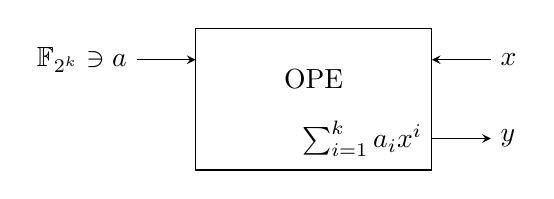
\begin{tikzpicture}[>=stealth]

    \node (OPE) at (8.5,0) {OPE};
    \draw (OPE) +(-1.5,-1.15) rectangle +(1.5,0.65);

    \draw [<-] (OPE) ++(-1.5,0.25) node [anchor=west] {} -- +(-0.75,0) node
    [anchor=east] {$\JWfieldGeneral \ni a$};

    \draw [<-] (OPE) ++(1.5,0.25) node [anchor=east] {} -- +(0.75,0) node
    [anchor=west] {$x$};

    \draw [->] (OPE) ++(1.5,-0.75) node [anchor=east] {$\sum_{i=1}^k a_ix^i$}
    -- +(0.75,0)
    node [anchor=west] {$y$};

  \end{tikzpicture}

  \caption{Graphical Representation of \JWfuncSymOPE}

\end{figure}

\begin{JWprotocol}%
  {\JWprotoSymOPE}%
  {Protocol: Oblivious Polynomial Evaluation}%
  {fig:proto-ope}

  Parametrized by the security parameter $k$ that specifies the field
  $\mathbb{F}_{2^k}$ and the maximal degree of the polynomial $n$.

  \JWprotoPhase{Setup:}

  \begin{JWprotoSteps}

  \item Upon input \JWmsgTP{Commit}{$a$} from the environment, \JWpOne{}
    verifies that $a \in \mathbb{F}_{2^k}^{n+1}$; else ignore that input. Next,
    \JWpOne{} generates the DRAC and sets up the OAFE functionality for the
    polynomial $f(x) = \sum_{i=0}^n a_ix^i$ (see section \ref{sec:OPE}).

  \item Finally, \JWpOne{} sends DRAC to \JWpTwo{}.

  \end{JWprotoSteps}


  \JWprotoPhase{Evaluation:}

  \begin{JWprotoSteps}

  \item Upon receiving the DRAC from \JWpOne{}, verify that there is no stored
    DRAC yet, else ignore that input. Next, \JWpTwo{} verifies the received
    input really it a DRAC, else ignore that input. Additionally it verifies
    that the DRAC encodes a function whose degree is less or equal than $n$ (see
    chapter \ref{sec:max-poly-degree}), else ignore the input. If the DRAC
    verification was successful, store the DRAC.

  \item Upon receiving input \JWmsgTP{Evaluate}{$x$} from the environment,
    verify that $x \in \mathbb{F}_{2^k}$, else ignore that input. If there is
    already a stored DRAC, continue at the next step, else wait for a stored
    DRAC.

  \item Next, \JWpTwo{} evaluates the DRAC. Because the OAFE functionality is
    set up by \JWpOne{}, during the evaluation it is possible that the OAFE
    functionality turns out to behave unexpectedly: It could decline needed
    evaluations and it could return vectors of unexpected shapes. In both cases
    always assume it would have returned all zero vectors of the expected shape.

  \item After the Evaluation, \JWpTwo{} adds both components of the last DRAV
    and queries a special final OAFE with that value. Again, assume the all zero
    vector is the OAFE behaves unexpectedly. The then received new value is the
    result of the computation $y = \sum_{i=1}^k a_ix^i$. Finally, output
    \JWmsgTP{Evaluated}{$y$} to the environment.

  \end{JWprotoSteps}

\end{JWprotocol}

% vim: set spell spelllang=en_us fileencoding=utf8 :


\JWlone{Correctness and Security of the Protocol}
\label{sec:security}

This chapter states and proofs the security of the protocol in the
\JWdef{Universal--Composability}{UC} framework by Ran Canetti \cite{canetti05}.
In the UC framework security is defined by comparing an \emph{ideal model} to a
\emph{real model}. The ideal model implements the intended functionality
\JWfuncSym{}{} safely by definition. The protocol under examination runs in the
real model. In the real model, there is an adversary $\mathcal{A}$ that controls
all corrupted parties.  In the ideal model, there is a simulator $\mathcal{S}$
that tries to mimic $\mathcal{A}$. An environment $\mathcal{Z}$ is plugged to
either the real or the ideal model and has to guess to which it's plugged to. A
protocol \JWprotoSym{}{} is an universally composable implementation of the
ideal functionality if for every adversary $\mathcal{A}$ there is a
simulator $\mathcal{S}$ such that for all environments $\mathcal{Z}$ the entire
view of $\mathcal{Z}$ in the real model (with \JWprotoSym{}{} and $\mathcal{A}$)
is statistically close to its view in the ideal model (with \JWfuncSym{}{} and
$\mathcal{S}$).

\begin{align*}
%
\forall \mathcal{A}\ \exists \mathcal{S}\ \forall \mathcal{Z} :
\text{ideal}\ \widetilde{=}\ \text{real}
%
\end{align*}

%
% SIMULATORS
%
\JWltwo{Simulators}
\label{sec:simulators}


% SIMULATOR S_DAVID(A)
\JWlthree{Simulator $\mathcal{S}_{\text{\JWpTwo{}}}(\mathcal{A})$}
\label{sec:simulator-david}

\paragraph{Setup Phase:}

\begin{itemize}

  \item Setup an emulated version of the given real model adversary
    \JWadv{} which especially impersonates the corrupted \JWpTwo{}.

  \item Setup emulated, honest \JWpOne{} labeled $\mathcal{G}$.

  \item Setup emulated, honest OAFE functionality labeled \JWfuncSymOAFE{}.

  \item Initialize $\mathcal{G}$ with a random polynomial of the parametrized
    degree $k$ and record the DRAC $C$ it generated.

  \item Wire $\mathcal{G}$, \JWfuncSymOAFE{} and \JWadv{} to each other
    and \JWadv{} to the environment as in the real model.

  \item Start the simulation by transitioning in the \emph{Processing Phase}.

\end{itemize}

\paragraph{Processing Phase:}

\begin{itemize}

  \item Intercept the adversary's (\JWadv{}) polynomial input $x$. This is
    trivial because it is the first message that \JWadv{} transmits to
    \JWfuncSymOAFE{} and was not ignored by \JWfuncSymOAFE{}. Notice, this is
    the initial DRAV encoding of the plain value $x$. Next, halt the simulation
    and evaluate the proper polynomial using the intercepted input $x$ and the
    ideal functionality \JWfuncSymOPEnp{} by sending it \JWmsgTP{Evaluate}{$x$}.

  \item Upon receiving \JWmsgTP{Evaluated}{$y$} from \JWfuncSymOPEnp{},
    calculate the value $\chi$ which an honest \JWpTwo{} would evaluate the last
    OAFE with. Because an honest \JWpTwo{} acts entirely deterministic, this
    calculates from the stored DRAC $C$, the OAFE parameters in \JWfuncSymOAFE,
    and the stored input $x$. Next, draw a random value $r$ and calculate $\psi
    = \frac{y-r}{\chi}$. Next, reconfigure the parameters of the last OAFE to
    $(\psi, r)$. The last OAFE then calculates the affine function $f(\eta) =
    \psi \cdot \eta + r$ which---when evaluated with $\chi$---calculates the
    result $y$ of the proper polynomial at the node $x$. Since any honest
    \JWpTwo{} evaluates the last OAFE with $\chi$, any honest \JWpTwo{} will
    receive the correct result $y = f(\chi) = \psi \cdot \chi + r =
    \frac{y-r}{\chi} \cdot \chi + r = y$. Any dishonest \JWpTwo{} will receive
    some random value depending on the random value $r$. Finally unhalt the
    simulation.

\end{itemize}


% SIMULATOR S_Goliath(A)
\JWlthree{Simulator $\mathcal{S}_{\text{Goliath}}(\mathcal{A})$}
\label{sec:simulator-goliath}

The setup phase is run as soon as the simulator starts.

\paragraph{Setup Phase:}

\begin{itemize}

  \item Setup emulated, honest \JWpTwo{} and OAFE functionality
    \JWfuncSymOAFE{}.

  \item Wire the given real model adversary \JWadv{} that impersonates \JWpOne{}
    with the emulated \JWpTwo{} and \JWfuncSymOAFE{}. Additionally wire \JWadv{}
    with the environment the way they would be wired in the real model.

\end{itemize}

\paragraph{Processing Phase:}

\begin{itemize}

  \item Upon the emulated OAFE functionality received the OAFE configuration and
    the emulated \JWpTwo{} received the DRAC, symbolically evaluate the
    polynomial that \JWadv{} described. During the symbolic evaluation, the OAFE
    functionality configuration could proof to be unfitting: \JWadv{} could
    have sent a configuration that allows too few OAFE evaluations or evaluates
    to vectors of wrong shape. In both cases, modify the configuration to return
    all zero vectors of the correct shape whenever the DRAC evaluation would
    fail otherwise.

  \item After having symbolically evaluated the polynomial encoded by \JWadv{},
    verify, that the polynomial has a degree that is less or equal than the
    parametrized degree $k$. If \JWadv{} submitted a polynomial of valid degree,
    store the polynomial's coefficients as $a \in \JWfieldGeneral^n$.  Next,
    upload that polynomial to the ideal functionality \JWfuncSymOPEnp{} by
    outputting \JWmsgTP{Commit}{$a$} to \JWfuncSymOPEnp{}.  If the polynomial
    was illegal, restart the simulator in the setup phase.  This restart is
    equivalent to ignoring the adversary's inputs.

\end{itemize}


%
% PROOF
%
\JWltwo{Security Proof}
\label{sec:proof}

The proof is a case distinction.


% CORRECTNESS --- BOTH PARTIES HONEST
\JWlthree{Correctness---Both Parties Honest}

\JWtodo{In richtigen Worten hinschreiben}

Easy, just works.



% BOTH PARTIES CORRUPTED
\JWlthree{Both Parties Corrupted}

\JWtodo{In richtigen Worten hinschreiben}

The case that both parties are corrupted is just an hypothetical case in the UC
model.


% CORRUPTED DAVID
\JWlthree{Corrupted \JWpTwo{}}

This chapter will proof the security of the proposed protocol \JWprotoSymOPE
in the Universal Composability (UC) framework \cite{canetti05} against both,
passive and active adversaries impersonating \JWpTwo{}. Passive adversaries are
adversaries which try to calculate additional information from intermediate
results, active adversaries additionally misuse the protocol in some
unpredictable way.

The protocol is trivially secure against passive adversaries impersonating
\JWpTwo{} because every value that gets transmitted to \JWpTwo{} is one--time
encrypted. The values which are sent to \JWpTwo{} are part of a DRAEs and DRAEs
only contain references to OAFEs and DRAVs. Chapter \ref{def:DRAV} proves (Lemma
\ref{lem:DRAV-random}) that DRAV only transport uncorrelated uniform randomness
to parties not in possession of the encryption keys. The OAFE evaluations lead
to further (one--time encrypted) DRAVs and radicals (see chapter
\ref{sec:sec-muls}) that are one--time encrypted as well. The simulator from
chapter \ref{sec:simulator-david} plays on this property and encodes a random
polynomial of the same degree that is used to test \JWpTwo{}'s honesty. In fact,
because every value is one--time encrypted, the protocol is perfectly secure
against any passive adversary.

For the security against an actively corrupted \JWpTwo{} a hybrid argument is
employed. The general idea is to transform an actively corrupted adversary
incrementally into a passively corrupted adversary and to show that the
statistical distance in the environment's view is negligible. For to random
variables $x$ and $y$ statistical distance $\Delta_S$ is denoted using the
following standard notation.

\begin{align*}
  %
  \Delta_S(x,y) = \frac{\sum_\alpha \left|Pr[x=\alpha] - Pr[y=\alpha]\right|}{2}
  %
\end{align*}

\noindent{}The first step is to attach a \emph{monitor module} between the
adversary \JWadv{} and the OAFE functionality \JWfuncSymOAFE{}. The monitor
module is parametrized by a transcript how an honest \JWpTwo{} would act. The
task of the module is to analyze the messages that \JWpTwo{} (impersonated by
the adversary) sends to the OAFE functionality. Upon the detection of a message
which does not match the honest transcript, it changes this message to match the
honest message. Additionally the monitor module intercepts the response to
changed message (sent by \JWfuncSymOAFE{}) and changes the response to some
value uniformly at random. The monitor module does this change only once, if the
adversary changes one of the following messages, the monitor module does no
further changes. The union of the adversary \JWadv{} and the
monitor module can be seen as a transformed adversary \JWadv{}' which is forging
(at the earliest) the message following the first message that \JWadv{}
illicitly changed. So, if \JWadv{} forges $n$ messages, \JWadv{}' forgest at
most $n-1$ messages.

The interesting part is the statistical distance of the environment's view
between \JWadv{} and \JWadv{}'. The message which \JWadv{} will receive from the
monitor module after having forged a message for the first time is uniform
randomness.  This will render some DRAV that is computed involving value in the
message to a non--well--formed DRAV with overwhelming probability. The
probability equals $1-1/|\mathbb{K}| = 1-1/2^k$ because exactly one element of
the finite field $\mathbb{K}$ matches its counterpart tuple component (see
chapter \ref{def:DRAV}). Therefore, the statistical distance
$\delta_{\mathcal{A},\mathcal{A}'}$ of the environment's view between \JWadv{}
and \JWadv{}' is:

\begin{align*}
  %
  \delta_{\mathcal{A},\mathcal{A}'} =
  \Delta_S(\text{view}_\mathcal{Z}(\mathcal{A}),
  \text{view}_\mathcal{Z}(\mathcal{A}'))
  \leq \frac{1}{|\mathbb{K}|}
  = \frac{1}{2^k}
  %
\end{align*}

\noindent{}This argument can be used inductively until the original adversary
\JWadv{} is transformed to a passive adversary $\mathcal{A}^*$ which does not
illicitly change any message. Because the triangle inequality holds for the
statistical distance and the maximal number of OAFEs used to evaluate a
polynomial of degree $n$ is in $O(n)$, the statistical distance between any
active adversary \JWadv{} and any passive adversary $\mathcal{A}^*$ is

\begin{align*}
  %
  \Delta_S(\text{view}_\mathcal{Z}(\mathcal{A}),
  \text{view}_\mathcal{Z}(\mathcal{A}^*))
  \leq \frac{O(n)}{2^k}
  %
\end{align*}

\noindent{}And because $k$ is the security parameter, the statistical distance
in the environment's view between any active adversary and any passive adversary
is negligible. As stated above, the protocol is perfectly secure against any
passive adversary and therefore information theoretically UC--secure against any
active adversary. \qed


% CORRUPTED GOLIATH
\JWlthree{Corrupted \JWpOne{}}

A corrupted \JWpOne{} has the following possibilities to cheat:

\begin{enumerate}

  \item Describe a polynomial with a degree other that the parametrized degree
    $k$.

  \item Configure the OAFE functionality in a way that the DRAC evaluation would
    fail because it assumes additional evaluation possibilities or vectors of
    other shapes.

  \item Send messages that do not describe a valid DRAC\@.

\end{enumerate}

\noindent{}Both, in the ideal model (running the simulator from
\ref{sec:simulator-goliath}) as well as in the real model (running the
\JWprotoSymOPE{} and the adversary) handle these possibilities indistinguishably
for any environment:

\begin{enumerate}

  \item The protocol and the simulator verify the polynomial's degree.
    Both ignore the input when the degree is other than parametrized.

  \item If the OAFE functionality is configured in a wrong way, both handle this
    case similarly: Vectors of wrong shapes are turned to the all zero vector of
    the correct shape. Missing OAFE evaluations are assumed to return the all
    zero vector of the expected shape.

  \item Messages that do not validly describe a DRAC are ignored.

\end{enumerate}

This assures any environment will not be able to distinguish between the real
and the ideal model.

% vim: set spell spelllang=en_us fileencoding=utf8 :


\JWlone{Implementation}
\label{sec:implementation}

In addition to the mathematical methods (chapter \ref{sec:methods}), the
protocol description (chapter \ref{sec:protocol}) and the security proof of the
protocol in the UC framework (chapter \ref{sec:security}), this thesis contains
an implementation of the protocol. The implementation is written in the lazy,
functional programming language \JWTLhaskell{}. More specifically \JWThaskell{}
as implemented by the major \JWThaskell{} compiler the \JWTXLghc{} (\JWTghc{})
version \JWTVghc{}.

The implementation was designed to match the descriptions in the above chapters
as closely as possible. The implementation implements Oblivious Polynomial
Evaluation as explained in chapter \ref{def:OPE}.

Even the Haskell data--types such as \JWcode{DRAC}, \JWcode{DRAE}, \JWcode{RAE},
\JWcode{LinearExpr} match the names of the constructs described in chapter
\ref{sec:methods}: DRACs (chapter \ref{def:DRAC}), (chapter \ref{def:DRAE}) and
linear expressions (named $\mathcal{C}$ in chapter \ref{def:DRAE}). For
practical reasons the program also features \JWcode{RAC} (Randomized Affine
Circuits) and \JWcode{RAE} (Randomized Affine Encodings) which are the same as
their \emph{dual} counterparts but split up by the components. So while running
the program two \JWcode{RAE}s are derived from one \JWcode{DRAE}.

As in chapter \ref{def:OPE}, the oblivious polynomial evaluation consists of
three parties: The tamper--proof hardware issuing party \JWpOne{} (executable
program called \JWBpOne{}), the receiving party \JWpTwo{} (\JWBpTwo{}) and the
tamper--proof hardware \JWtoken{} (\JWBtoken{}). The individual programs talk to
each other using TCP/IP networking. The \JWtoken{} implements the OAFE
functionality \JWfuncSym{seq-ot}{OAFE} as provided by the David \& Goliath
protocol \cite{davidgoliath}. The \JWtoken{} does not actually implement the
David \& Goliath protocol but only it's interface. A real implementation using a
tamper--proof hardware token is left open to potential future works.


%
% COMMUNICATION CHANNELS
%
\JWltwo{Communication Channels and Their TCP Ports}
\label{sec:communication-channels}


% GOLIATH TO TOKEN
\JWlthree{\JWpOne{} To \JWtoken{}}
\label{sec:comm:goliath2Token}

On TCP port \JWport{23120} \JWpOne{} initiates a connection to the \JWtoken{}.
This connection is used to transfer the OAFE configuration to the tamper--proof
hardware token.


% DAVID TO TOKEN
\JWlthree{\JWpTwo{} To \JWtoken{}}
\label{sec:comm:david2token}

On TCP port \JWport{23021} \JWpTwo{} initiates a connection to the \JWtoken{}.
This connection is used to evaluate the OAFEs. \JWpTwo{} sends a tells which
OAFE to evaluate and its value, the \JWtoken{} then replies with a vector
consisting of the evaluated linear expressions.


% GOLIATH TO DAVID
\JWlthree{\JWpOne{} To \JWpTwo{}}
\label{sec:comm:goliath2david}

On TCP port \JWport{23102} \JWpOne{} initiates a connection to \JWpTwo{}. This
connection is a stream of \JWpTwo{} DRAEs (in fact \JWcode{RAE}s) assigned to
variables, that \JWpTwo{} will evaluate one after the other in the order
\JWpOne{} has sent them.


% DAVID TO GOLIATH
\JWlthree{\JWpTwo{} To \JWpOne{}}
\label{sec:comm:david2goliath}

On TCP port \JWport{23201} \JWpTwo{} initiates a connection to \JWpOne{}. This
connection is not necessary for the protocol itself but is used to exchange
settings between \JWpOne{} and \JWpTwo{}. \JWpOne{} tells \JWpTwo{} the host
name and the TCP port of the \JWtoken{} and \JWpTwo{} tells \JWpOne{} the port
on which \JWpTwo{} accepts the DRAE stream.


%
% DIFFERENCES BETWEEN IMPLEMENTATION AND WRITING
%
\JWltwo{Differences Between the Implementation and this Writing}
\label{sec:implementation-differences}

\begin{itemize}

\item In writing there are no \JWcode{RAE}s

\item Communication Channel from \JWpTwo{} to \JWpOne{}
(\ref{sec:comm:david2goliath})

\item THERE IS NOT TAMPER-PROOF HARWARE TOKEN

\end{itemize}


%
% IMPLEMENTATION DETAILS
%
\JWltwo{Implementation Details}
\label{sec:implementation-details}

% Calculations in Finite Fields
\JWlthree{Calculations in Finite Fields}

For the calculation in the finite fields (chapter \ref{sec:field}) the
\JWTcpp{} library \JWTLntl{} (\emph{Number Theory Library}) has been interfaced
to \JWThaskell{} for the purpose of developing the implementation of this
thesis. The interface has been developed using \JWThaskell{}'s \JWdef{Foreign
Function Interface}{FFI} \cite{haskell2010} and \JWdef{C $\longrightarrow$
Haskell}{C2Hs} \cite{c2hs}. Prior to interfacing the library to Haskell a very
lightweight \JWTc{} wrapper has been developed because the library is written in
\JWTcpp{} which cannot directly be interfaced using the FFI.


% Testing Correctness
\JWlthree{Testing the Correctness of the Implementation}

The correctness of the implementation has not been proofed since that is not
feasible for complex programs. Instead of a real proof, the implementation
has been tested using the specification--driven automatic \JWThaskell{} testing
tool \JWTquickcheck{} \cite{quickcheck} and the classic unit test approach of
\JWTLhunit{}.


% Randomness
\JWlthree{Cryptographic Randomness}

The random numbers needed for the implementation of this thesis are generated
using \JWTLmonadcryptorandom{}.


% Communication Layer
\JWlthree{Communication Layer}

The communication layer between the different binaries is driven by the
schrieblesque \JWTXLprotobuf{}.


% Other Libraries
\JWlthree{Other Libraries}

This thesis uses a lot of other libraries mainly from \JWTLhackage{}. The
complete list of packages can be extracted from the file
\JWpath{diplomarbeit.cabal} that comes with the source code of this thesis.


% Build System
\JWlthree{Build System and Building}

The implementation can be easily built using \JWTLcabal{} by typing:

\begin{lstlisting}

cd diplomarbeit/
cabal install --only-dependencies
cabal configure
cabal build

\end{lstlisting}


%
% DOCUMENTATION
%
\JWltwo{Documentation}
\label{sec:implementation-doc}

The implementation is documented using \JWTLhaddock{}.

\JWtodo{Add link to Haddock doc}


%
% CODE AVAILABILITY
%
\JWltwo{Code Availability}
\label{sec:code-availability}

All of the code is open--sourced and available at...
\JWtodo{Add link to GitHub repo}


% vim: set spell spelllang=en_us fileencoding=utf8 :


\JWlone{Evaluation and Conclusion}
\label{sec:evaluation}

This part evaluates the computational complexity of the methodology and the
performance of the implementation. Additionally, this thesis' contribution and
the open questions are exposed in the following.

%
% TEST SETUP
%
\JWltwo{Test Setup}
\label{sec:test-setup}

\JWlthree{Test Machines}
\label{sec:test-machines}

Both test machines are regular home computer systems thus the benchmarks were
not run under laboratory conditions. Though, most background services and other
programs that could interfere with the benchmarks have been stopped. The
implementation has been compiled using full optimizations turned on
(\JWcmd{cabal configure --ghc-options=-O3}). To work out the computing time
taken for the implementation of the protocol itself, the protocol implementation
is evaluated using two different implementation of finite field calculations.
The first implementation is a C++ library (see chapter
\ref{sec:finite-field-calcs}) for calculations in $\mathbb{F}_{2^{256}}$ and the
second implementation is a \JWThaskell{} library which calculates in the prime
field $\mathbb{F}_{97}$.


\JWlfour*{Test Machine 1}

\emph{Dell Latitude D620} running \emph{Debian GNU/Linux} on kernel version
\emph{3.1.7, 32--bit}. The machine is powered by a \emph{Intel\TReg{} Core Duo
T2400} dual core processor at \emph{1.83 GHz}. It has \emph{2 GB} system memory.


\JWlfour*{Test Machine 2}

\emph{Apple Mac mini} (\texttt{Macmini 3,1}) running \emph{MacOS X 10.7.5
(Lion), 64--bit}. The machine is powered by a \emph{Intel\TReg{} Core 2 Duo}
dual core processor at \emph{2.26 GHz}. It has \emph{8 GB} system memory.

\JWlthree{Benchmarking Process}

Both machines run the three programs (\JWBpOne{}, \JWBpTwo{}, \JWBtoken{})
simultaneously, the programs are compiled single--threaded. The programs
communicate to each other using local TCP/IP networking. Chapter
\ref{sec:communication-channels} has an in depth description about the
communication that takes part in the implementation that comes with this thesis.
The running time includes the DRAC building and transmitting, the OAFE
configuration and the successful evaluation of a random polynomial. The
polynomial is evaluated using \emph{Horner's rule}\cite{cormen01}. The data
points in all figures and tables was obtained by taking the median of
running the same benchmark five times in a row (preceded by a non--accounted
warm--up run).


%
% COMPUTATIONAL COMPLEXITY
%
\JWltwo{Computational Complexity}
\label{sec:comp-complexity}

Ordinary evaluation of a polynomial of degree $n$ using \emph{Horner's rule} is
in $\Theta(n)$ \cite{cormen01}. Despite the complex technique presented in this
thesis the overall evaluation time is still in $\Theta(n)$. This is true for
both, the theoretical examination and the implementation. Figure
\ref{fig:poly-deg-t} and table \ref{tab:poly-deg-t} show this for the finite
field $\mathbb{F}_{97}$ (implementation from the \JWTLhaskellForMaths{}
package). The implementation for the field $\mathbb{F}_{2^{256}}$ does not seem
to have linear time complexity. This is caused by the unoptimal implementation
and the Haskell binding of the library used for the calculations in
$\mathbb{F}_{2^{256}}$. It is problematic that the library includes a rather
complex routine for object destruction that takes most of the evaluation time.
Root of the problem is that functional languages prefer immutable (unchangeable)
objects with very fast construction/destruction and the C++ library that is
interfaced is optimized for as few constructions/destructions as possible and
the use of mutable objects. The phenomenon that is observable when using this
library is that the garbage collector is taking up most of the running time (up
to $85\%$) waiting for the library destruction routine. For high performance
(such as the pure Haskell implementation for $\mathbb{F}_{97}$) another library
should be interfaced or developed entirely in Haskell, but this is not the main
concern of this thesis. Futher details are covered in chapter
\ref{sec:finite-field-calcs}. For lower degrees, the current implementation for
$\mathbb{F}_{2^{256}}$ has linear time complexity. Figure
\ref{fig:poly-deg-t-small} and table \ref{tab:poly-deg-t-small} show this. It is
also noteworthy that the first test machine (see chapter
\ref{sec:test-machines}) outperforms the second test machine despite the
inferior hardware. The cause has not been investigated, a possible cause could
be that the 64--bit \JWTghc{} runtime seems to be slower (at least on Apple
Macs)\cite{lentczner11}.


% F97 vs. F2Pow256 and Linux vs. Mac
\begin{figure}[ht]
  \centering
  % Created by tikzDevice version 0.6.2-92-0ad2792 on 2012-12-13 16:37:48
% !TEX encoding = UTF-8 Unicode
\begin{tikzpicture}[x=1pt,y=1pt]
\definecolor[named]{fillColor}{rgb}{1.00,1.00,1.00}
\path[use as bounding box,fill=fillColor,fill opacity=0.00] (0,0) rectangle (433.62,505.89);
\begin{scope}
\path[clip] ( 49.20, 61.20) rectangle (408.42,456.69);
\definecolor[named]{drawColor}{rgb}{0.00,0.00,0.00}

\path[draw=drawColor,line width= 0.4pt,line join=round,line cap=round] ( 62.50, 81.16) --
	( 80.01, 86.96) --
	( 97.52, 92.76) --
	(115.02, 98.24) --
	(132.53,103.40) --
	(150.03,108.85) --
	(167.54,114.59) --
	(185.05,119.88) --
	(202.55,125.55) --
	(220.06,131.19) --
	(237.56,136.81) --
	(255.07,142.43) --
	(272.57,148.18) --
	(290.08,153.49) --
	(307.59,159.59) --
	(325.09,165.16) --
	(342.60,171.23) --
	(360.10,176.98) --
	(377.61,183.36) --
	(395.12,189.02);

\path[draw=drawColor,line width= 0.4pt,line join=round,line cap=round] ( 62.50, 81.16) circle (  2.25);

\path[draw=drawColor,line width= 0.4pt,line join=round,line cap=round] ( 80.01, 86.96) circle (  2.25);

\path[draw=drawColor,line width= 0.4pt,line join=round,line cap=round] ( 97.52, 92.76) circle (  2.25);

\path[draw=drawColor,line width= 0.4pt,line join=round,line cap=round] (115.02, 98.24) circle (  2.25);

\path[draw=drawColor,line width= 0.4pt,line join=round,line cap=round] (132.53,103.40) circle (  2.25);

\path[draw=drawColor,line width= 0.4pt,line join=round,line cap=round] (150.03,108.85) circle (  2.25);

\path[draw=drawColor,line width= 0.4pt,line join=round,line cap=round] (167.54,114.59) circle (  2.25);

\path[draw=drawColor,line width= 0.4pt,line join=round,line cap=round] (185.05,119.88) circle (  2.25);

\path[draw=drawColor,line width= 0.4pt,line join=round,line cap=round] (202.55,125.55) circle (  2.25);

\path[draw=drawColor,line width= 0.4pt,line join=round,line cap=round] (220.06,131.19) circle (  2.25);

\path[draw=drawColor,line width= 0.4pt,line join=round,line cap=round] (237.56,136.81) circle (  2.25);

\path[draw=drawColor,line width= 0.4pt,line join=round,line cap=round] (255.07,142.43) circle (  2.25);

\path[draw=drawColor,line width= 0.4pt,line join=round,line cap=round] (272.57,148.18) circle (  2.25);

\path[draw=drawColor,line width= 0.4pt,line join=round,line cap=round] (290.08,153.49) circle (  2.25);

\path[draw=drawColor,line width= 0.4pt,line join=round,line cap=round] (307.59,159.59) circle (  2.25);

\path[draw=drawColor,line width= 0.4pt,line join=round,line cap=round] (325.09,165.16) circle (  2.25);

\path[draw=drawColor,line width= 0.4pt,line join=round,line cap=round] (342.60,171.23) circle (  2.25);

\path[draw=drawColor,line width= 0.4pt,line join=round,line cap=round] (360.10,176.98) circle (  2.25);

\path[draw=drawColor,line width= 0.4pt,line join=round,line cap=round] (377.61,183.36) circle (  2.25);

\path[draw=drawColor,line width= 0.4pt,line join=round,line cap=round] (395.12,189.02) circle (  2.25);
\end{scope}
\begin{scope}
\path[clip] (  0.00,  0.00) rectangle (433.62,505.89);
\definecolor[named]{drawColor}{rgb}{0.00,0.00,0.00}

\path[draw=drawColor,line width= 0.4pt,line join=round,line cap=round] (115.02, 61.20) -- (395.12, 61.20);

\path[draw=drawColor,line width= 0.4pt,line join=round,line cap=round] (115.02, 61.20) -- (115.02, 55.20);

\path[draw=drawColor,line width= 0.4pt,line join=round,line cap=round] (185.05, 61.20) -- (185.05, 55.20);

\path[draw=drawColor,line width= 0.4pt,line join=round,line cap=round] (255.07, 61.20) -- (255.07, 55.20);

\path[draw=drawColor,line width= 0.4pt,line join=round,line cap=round] (325.09, 61.20) -- (325.09, 55.20);

\path[draw=drawColor,line width= 0.4pt,line join=round,line cap=round] (395.12, 61.20) -- (395.12, 55.20);

\node[text=drawColor,anchor=base,inner sep=0pt, outer sep=0pt, scale=  1.00] at (115.02, 39.60) {2000};

\node[text=drawColor,anchor=base,inner sep=0pt, outer sep=0pt, scale=  1.00] at (185.05, 39.60) {4000};

\node[text=drawColor,anchor=base,inner sep=0pt, outer sep=0pt, scale=  1.00] at (255.07, 39.60) {6000};

\node[text=drawColor,anchor=base,inner sep=0pt, outer sep=0pt, scale=  1.00] at (325.09, 39.60) {8000};

\node[text=drawColor,anchor=base,inner sep=0pt, outer sep=0pt, scale=  1.00] at (395.12, 39.60) {10000};

\path[draw=drawColor,line width= 0.4pt,line join=round,line cap=round] ( 49.20, 75.85) -- ( 49.20,439.02);

\path[draw=drawColor,line width= 0.4pt,line join=round,line cap=round] ( 49.20, 75.85) -- ( 43.20, 75.85);

\path[draw=drawColor,line width= 0.4pt,line join=round,line cap=round] ( 49.20,136.38) -- ( 43.20,136.38);

\path[draw=drawColor,line width= 0.4pt,line join=round,line cap=round] ( 49.20,196.90) -- ( 43.20,196.90);

\path[draw=drawColor,line width= 0.4pt,line join=round,line cap=round] ( 49.20,257.43) -- ( 43.20,257.43);

\path[draw=drawColor,line width= 0.4pt,line join=round,line cap=round] ( 49.20,317.96) -- ( 43.20,317.96);

\path[draw=drawColor,line width= 0.4pt,line join=round,line cap=round] ( 49.20,378.49) -- ( 43.20,378.49);

\path[draw=drawColor,line width= 0.4pt,line join=round,line cap=round] ( 49.20,439.02) -- ( 43.20,439.02);

\node[text=drawColor,rotate= 90.00,anchor=base,inner sep=0pt, outer sep=0pt, scale=  1.00] at ( 34.80, 75.85) {0};

\node[text=drawColor,rotate= 90.00,anchor=base,inner sep=0pt, outer sep=0pt, scale=  1.00] at ( 34.80,136.38) {20};

\node[text=drawColor,rotate= 90.00,anchor=base,inner sep=0pt, outer sep=0pt, scale=  1.00] at ( 34.80,196.90) {40};

\node[text=drawColor,rotate= 90.00,anchor=base,inner sep=0pt, outer sep=0pt, scale=  1.00] at ( 34.80,257.43) {60};

\node[text=drawColor,rotate= 90.00,anchor=base,inner sep=0pt, outer sep=0pt, scale=  1.00] at ( 34.80,317.96) {80};

\node[text=drawColor,rotate= 90.00,anchor=base,inner sep=0pt, outer sep=0pt, scale=  1.00] at ( 34.80,378.49) {100};

\node[text=drawColor,rotate= 90.00,anchor=base,inner sep=0pt, outer sep=0pt, scale=  1.00] at ( 34.80,439.02) {120};

\path[draw=drawColor,line width= 0.4pt,line join=round,line cap=round] ( 49.20, 61.20) --
	(408.42, 61.20) --
	(408.42,456.69) --
	( 49.20,456.69) --
	( 49.20, 61.20);
\end{scope}
\begin{scope}
\path[clip] (  0.00,  0.00) rectangle (433.62,505.89);
\definecolor[named]{drawColor}{rgb}{0.00,0.00,0.00}

\node[text=drawColor,anchor=base,inner sep=0pt, outer sep=0pt, scale=  1.00] at (228.81, 15.60) {Polynomial Degree};

\node[text=drawColor,rotate= 90.00,anchor=base,inner sep=0pt, outer sep=0pt, scale=  1.00] at ( 10.80,258.94) {Running Time [s]};
\end{scope}
\begin{scope}
\path[clip] ( 49.20, 61.20) rectangle (408.42,456.69);
\definecolor[named]{drawColor}{rgb}{0.00,0.00,0.00}

\path[draw=drawColor,line width= 0.4pt,dash pattern=on 4pt off 4pt ,line join=round,line cap=round] ( 62.50, 83.08) --
	( 80.01, 94.10) --
	( 97.52,106.59) --
	(115.02,121.79) --
	(132.53,138.50) --
	(150.03,153.20) --
	(167.54,172.63) --
	(185.05,196.68) --
	(202.55,218.84) --
	(220.06,243.66) --
	(237.56,268.01) --
	(255.07,294.64) --
	(272.57,333.65) --
	(290.08,359.40) --
	(307.59,391.29) --
	(325.09,431.39) --
	(342.60,462.77) --
	(358.93,505.89);

\path[draw=drawColor,line width= 0.4pt,line join=round,line cap=round] ( 62.50, 83.08) circle (  2.25);

\path[draw=drawColor,line width= 0.4pt,line join=round,line cap=round] ( 80.01, 94.10) circle (  2.25);

\path[draw=drawColor,line width= 0.4pt,line join=round,line cap=round] ( 97.52,106.59) circle (  2.25);

\path[draw=drawColor,line width= 0.4pt,line join=round,line cap=round] (115.02,121.79) circle (  2.25);

\path[draw=drawColor,line width= 0.4pt,line join=round,line cap=round] (132.53,138.50) circle (  2.25);

\path[draw=drawColor,line width= 0.4pt,line join=round,line cap=round] (150.03,153.20) circle (  2.25);

\path[draw=drawColor,line width= 0.4pt,line join=round,line cap=round] (167.54,172.63) circle (  2.25);

\path[draw=drawColor,line width= 0.4pt,line join=round,line cap=round] (185.05,196.68) circle (  2.25);

\path[draw=drawColor,line width= 0.4pt,line join=round,line cap=round] (202.55,218.84) circle (  2.25);

\path[draw=drawColor,line width= 0.4pt,line join=round,line cap=round] (220.06,243.66) circle (  2.25);

\path[draw=drawColor,line width= 0.4pt,line join=round,line cap=round] (237.56,268.01) circle (  2.25);

\path[draw=drawColor,line width= 0.4pt,line join=round,line cap=round] (255.07,294.64) circle (  2.25);

\path[draw=drawColor,line width= 0.4pt,line join=round,line cap=round] (272.57,333.65) circle (  2.25);

\path[draw=drawColor,line width= 0.4pt,line join=round,line cap=round] (290.08,359.40) circle (  2.25);

\path[draw=drawColor,line width= 0.4pt,line join=round,line cap=round] (307.59,391.29) circle (  2.25);

\path[draw=drawColor,line width= 0.4pt,line join=round,line cap=round] (325.09,431.39) circle (  2.25);

\path[draw=drawColor,line width= 0.4pt,line join=round,line cap=round] (342.60,462.77) circle (  2.25);

\path[draw=drawColor,line width= 0.4pt,dash pattern=on 1pt off 3pt ,line join=round,line cap=round] ( 62.50, 79.69) --
	( 80.01, 84.09) --
	( 97.52, 88.43) --
	(115.02, 92.65) --
	(132.53, 97.15) --
	(150.03,101.46) --
	(167.54,106.21) --
	(185.05,110.46) --
	(202.55,114.60) --
	(220.06,118.68) --
	(237.56,123.01) --
	(255.07,127.54) --
	(272.57,131.97) --
	(290.08,136.40) --
	(307.59,141.60) --
	(325.09,145.83) --
	(342.60,150.73) --
	(360.10,155.29) --
	(377.61,160.45) --
	(395.12,165.60);

\path[draw=drawColor,line width= 0.4pt,line join=round,line cap=round] ( 60.51, 77.70) rectangle ( 64.50, 81.69);

\path[draw=drawColor,line width= 0.4pt,line join=round,line cap=round] ( 78.02, 82.10) rectangle ( 82.00, 86.09);

\path[draw=drawColor,line width= 0.4pt,line join=round,line cap=round] ( 95.52, 86.43) rectangle ( 99.51, 90.42);

\path[draw=drawColor,line width= 0.4pt,line join=round,line cap=round] (113.03, 90.66) rectangle (117.02, 94.64);

\path[draw=drawColor,line width= 0.4pt,line join=round,line cap=round] (130.53, 95.16) rectangle (134.52, 99.14);

\path[draw=drawColor,line width= 0.4pt,line join=round,line cap=round] (148.04, 99.47) rectangle (152.03,103.46);

\path[draw=drawColor,line width= 0.4pt,line join=round,line cap=round] (165.55,104.22) rectangle (169.53,108.21);

\path[draw=drawColor,line width= 0.4pt,line join=round,line cap=round] (183.05,108.47) rectangle (187.04,112.46);

\path[draw=drawColor,line width= 0.4pt,line join=round,line cap=round] (200.56,112.61) rectangle (204.55,116.60);

\path[draw=drawColor,line width= 0.4pt,line join=round,line cap=round] (218.06,116.69) rectangle (222.05,120.67);

\path[draw=drawColor,line width= 0.4pt,line join=round,line cap=round] (235.57,121.02) rectangle (239.56,125.01);

\path[draw=drawColor,line width= 0.4pt,line join=round,line cap=round] (253.07,125.55) rectangle (257.06,129.54);

\path[draw=drawColor,line width= 0.4pt,line join=round,line cap=round] (270.58,129.97) rectangle (274.57,133.96);

\path[draw=drawColor,line width= 0.4pt,line join=round,line cap=round] (288.09,134.41) rectangle (292.07,138.39);

\path[draw=drawColor,line width= 0.4pt,line join=round,line cap=round] (305.59,139.61) rectangle (309.58,143.59);

\path[draw=drawColor,line width= 0.4pt,line join=round,line cap=round] (323.10,143.84) rectangle (327.09,147.82);

\path[draw=drawColor,line width= 0.4pt,line join=round,line cap=round] (340.60,148.74) rectangle (344.59,152.73);

\path[draw=drawColor,line width= 0.4pt,line join=round,line cap=round] (358.11,153.30) rectangle (362.10,157.29);

\path[draw=drawColor,line width= 0.4pt,line join=round,line cap=round] (375.62,158.45) rectangle (379.60,162.44);

\path[draw=drawColor,line width= 0.4pt,line join=round,line cap=round] (393.12,163.61) rectangle (397.11,167.60);

\path[draw=drawColor,line width= 0.4pt,dash pattern=on 1pt off 3pt on 4pt off 3pt ,line join=round,line cap=round] ( 62.50, 80.51) --
	( 80.01, 85.81) --
	( 97.52, 92.92) --
	(115.02,101.55) --
	(132.53,113.64) --
	(150.03,125.20) --
	(167.54,136.55) --
	(185.05,151.97) --
	(202.55,165.19) --
	(220.06,181.99) --
	(237.56,199.60) --
	(255.07,221.58) --
	(272.57,239.55) --
	(290.08,259.92) --
	(307.59,281.82) --
	(325.09,307.99) --
	(342.60,339.54) --
	(360.10,367.96) --
	(377.61,394.30) --
	(395.12,420.66);

\path[draw=drawColor,line width= 0.4pt,line join=round,line cap=round] ( 60.51, 78.52) rectangle ( 64.50, 82.51);

\path[draw=drawColor,line width= 0.4pt,line join=round,line cap=round] ( 78.02, 83.82) rectangle ( 82.00, 87.80);

\path[draw=drawColor,line width= 0.4pt,line join=round,line cap=round] ( 95.52, 90.92) rectangle ( 99.51, 94.91);

\path[draw=drawColor,line width= 0.4pt,line join=round,line cap=round] (113.03, 99.55) rectangle (117.02,103.54);

\path[draw=drawColor,line width= 0.4pt,line join=round,line cap=round] (130.53,111.65) rectangle (134.52,115.64);

\path[draw=drawColor,line width= 0.4pt,line join=round,line cap=round] (148.04,123.21) rectangle (152.03,127.20);

\path[draw=drawColor,line width= 0.4pt,line join=round,line cap=round] (165.55,134.55) rectangle (169.53,138.54);

\path[draw=drawColor,line width= 0.4pt,line join=round,line cap=round] (183.05,149.98) rectangle (187.04,153.96);

\path[draw=drawColor,line width= 0.4pt,line join=round,line cap=round] (200.56,163.20) rectangle (204.55,167.19);

\path[draw=drawColor,line width= 0.4pt,line join=round,line cap=round] (218.06,179.99) rectangle (222.05,183.98);

\path[draw=drawColor,line width= 0.4pt,line join=round,line cap=round] (235.57,197.60) rectangle (239.56,201.59);

\path[draw=drawColor,line width= 0.4pt,line join=round,line cap=round] (253.07,219.58) rectangle (257.06,223.57);

\path[draw=drawColor,line width= 0.4pt,line join=round,line cap=round] (270.58,237.55) rectangle (274.57,241.54);

\path[draw=drawColor,line width= 0.4pt,line join=round,line cap=round] (288.09,257.93) rectangle (292.07,261.91);

\path[draw=drawColor,line width= 0.4pt,line join=round,line cap=round] (305.59,279.82) rectangle (309.58,283.81);

\path[draw=drawColor,line width= 0.4pt,line join=round,line cap=round] (323.10,306.00) rectangle (327.09,309.99);

\path[draw=drawColor,line width= 0.4pt,line join=round,line cap=round] (340.60,337.54) rectangle (344.59,341.53);

\path[draw=drawColor,line width= 0.4pt,line join=round,line cap=round] (358.11,365.96) rectangle (362.10,369.95);

\path[draw=drawColor,line width= 0.4pt,line join=round,line cap=round] (375.62,392.30) rectangle (379.60,396.29);

\path[draw=drawColor,line width= 0.4pt,line join=round,line cap=round] (393.12,418.67) rectangle (397.11,422.65);

\path[draw=drawColor,line width= 0.4pt,line join=round,line cap=round] ( 55.50,439.02) rectangle (204.10,379.02);

\path[draw=drawColor,line width= 0.4pt,line join=round,line cap=round] ( 58.20,427.02) -- ( 76.20,427.02);

\path[draw=drawColor,line width= 0.4pt,dash pattern=on 4pt off 4pt ,line join=round,line cap=round] ( 58.20,415.02) -- ( 76.20,415.02);

\path[draw=drawColor,line width= 0.4pt,dash pattern=on 1pt off 3pt ,line join=round,line cap=round] ( 58.20,403.02) -- ( 76.20,403.02);

\path[draw=drawColor,line width= 0.4pt,dash pattern=on 1pt off 3pt on 4pt off 3pt ,line join=round,line cap=round] ( 58.20,391.02) -- ( 76.20,391.02);

\path[draw=drawColor,line width= 0.4pt,line join=round,line cap=round] ( 67.20,427.02) circle (  2.25);

\path[draw=drawColor,line width= 0.4pt,line join=round,line cap=round] ( 67.20,415.02) circle (  2.25);

\path[draw=drawColor,line width= 0.4pt,line join=round,line cap=round] ( 65.21,401.02) rectangle ( 69.20,405.01);

\path[draw=drawColor,line width= 0.4pt,line join=round,line cap=round] ( 65.21,389.02) rectangle ( 69.20,393.01);

\node[text=drawColor,anchor=base west,inner sep=0pt, outer sep=0pt, scale=  1.00] at ( 85.20,423.57) {Test Machine 1, $\mathbb{F}_{97}\qquad$};

\node[text=drawColor,anchor=base west,inner sep=0pt, outer sep=0pt, scale=  1.00] at ( 85.20,411.57) {Test Machine 1, $\mathbb{F}_{2^{256}}\qquad$};

\node[text=drawColor,anchor=base west,inner sep=0pt, outer sep=0pt, scale=  1.00] at ( 85.20,399.57) {Test Machine 2, $\mathbb{F}_{97}\qquad$};

\node[text=drawColor,anchor=base west,inner sep=0pt, outer sep=0pt, scale=  1.00] at ( 85.20,387.57) {Test Machine 2, $\mathbb{F}_{2^{256}}\qquad$};
\end{scope}
\end{tikzpicture}

  \caption{Evaluation Time of Polynomial by Degree}
  \label{fig:poly-deg-t}
\end{figure}

\begin{table}[ht]
  \centering
  \begin{tabular}{|c|c|c|}
    Polynomial Degree & Running Time $\mathbb{F}_{97}$ [s] & Running Time
    $\mathbb{F}_{2^{256}}$ [s]\\
    %
      500 &  1.754 &   2.389 \\
     1000 &  3.673 &   6.032 \\
     1500 &  5.587 &  10.159 \\
     2000 &  7.400 &  15.179 \\
     2500 &  9.104 &  20.702 \\
     3000 & 10.905 &  25.560 \\
     3500 & 12.800 &  31.978 \\
     4000 & 14.549 &  39.926 \\
     4500 & 16.422 &  47.248 \\
     5000 & 18.288 &  55.450 \\
     5500 & 20.142 &  63.496 \\
     6000 & 22.000 &  72.293 \\
     6500 & 23.901 &  85.184 \\
     7000 & 25.654 &  93.694 \\
     7500 & 27.670 & 104.231 \\
     8000 & 29.510 & 117.480 \\
     8500 & 31.518 & 127.848 \\
     9000 & 33.417 & 143.123 \\
     9500 & 35.525 & 156.820 \\
    10000 & 37.395 & 172.216 \\

  \end{tabular}
  \caption{Evaluation Time of Polynomials by Degree on Test Machine 1}
  \label{tab:poly-deg-t}
\end{table}

\begin{figure}[ht]
  \centering
  % Created by tikzDevice version 0.6.2-92-0ad2792 on 2012-12-16 13:16:22
% !TEX encoding = UTF-8 Unicode
\begin{tikzpicture}[x=1pt,y=1pt]
\definecolor[named]{fillColor}{rgb}{1.00,1.00,1.00}
\path[use as bounding box,fill=fillColor,fill opacity=0.00] (0,0) rectangle (433.62,216.81);
\begin{scope}
\path[clip] ( 49.20, 61.20) rectangle (408.42,167.61);
\definecolor[named]{drawColor}{rgb}{0.00,0.00,0.00}

\path[draw=drawColor,line width= 0.4pt,line join=round,line cap=round] ( 62.50, 65.14) --
	( 95.77, 71.74) --
	(129.03, 79.45) --
	(162.29, 88.09) --
	(195.55, 96.55) --
	(228.81,106.43) --
	(262.07,116.31) --
	(295.33,127.74) --
	(328.59,138.15) --
	(361.85,149.05) --
	(395.12,163.67);

\path[draw=drawColor,line width= 0.4pt,line join=round,line cap=round] ( 62.50, 65.14) circle (  2.25);

\path[draw=drawColor,line width= 0.4pt,line join=round,line cap=round] ( 95.77, 71.74) circle (  2.25);

\path[draw=drawColor,line width= 0.4pt,line join=round,line cap=round] (129.03, 79.45) circle (  2.25);

\path[draw=drawColor,line width= 0.4pt,line join=round,line cap=round] (162.29, 88.09) circle (  2.25);

\path[draw=drawColor,line width= 0.4pt,line join=round,line cap=round] (195.55, 96.55) circle (  2.25);

\path[draw=drawColor,line width= 0.4pt,line join=round,line cap=round] (228.81,106.43) circle (  2.25);

\path[draw=drawColor,line width= 0.4pt,line join=round,line cap=round] (262.07,116.31) circle (  2.25);

\path[draw=drawColor,line width= 0.4pt,line join=round,line cap=round] (295.33,127.74) circle (  2.25);

\path[draw=drawColor,line width= 0.4pt,line join=round,line cap=round] (328.59,138.15) circle (  2.25);

\path[draw=drawColor,line width= 0.4pt,line join=round,line cap=round] (361.85,149.05) circle (  2.25);

\path[draw=drawColor,line width= 0.4pt,line join=round,line cap=round] (395.12,163.67) circle (  2.25);
\end{scope}
\begin{scope}
\path[clip] (  0.00,  0.00) rectangle (433.62,216.81);
\definecolor[named]{drawColor}{rgb}{0.00,0.00,0.00}

\path[draw=drawColor,line width= 0.4pt,line join=round,line cap=round] ( 62.50, 61.20) -- (395.12, 61.20);

\path[draw=drawColor,line width= 0.4pt,line join=round,line cap=round] ( 62.50, 61.20) -- ( 62.50, 55.20);

\path[draw=drawColor,line width= 0.4pt,line join=round,line cap=round] (129.03, 61.20) -- (129.03, 55.20);

\path[draw=drawColor,line width= 0.4pt,line join=round,line cap=round] (195.55, 61.20) -- (195.55, 55.20);

\path[draw=drawColor,line width= 0.4pt,line join=round,line cap=round] (262.07, 61.20) -- (262.07, 55.20);

\path[draw=drawColor,line width= 0.4pt,line join=round,line cap=round] (328.59, 61.20) -- (328.59, 55.20);

\path[draw=drawColor,line width= 0.4pt,line join=round,line cap=round] (395.12, 61.20) -- (395.12, 55.20);

\node[text=drawColor,anchor=base,inner sep=0pt, outer sep=0pt, scale=  1.00] at ( 62.50, 39.60) {0};

\node[text=drawColor,anchor=base,inner sep=0pt, outer sep=0pt, scale=  1.00] at (129.03, 39.60) {100};

\node[text=drawColor,anchor=base,inner sep=0pt, outer sep=0pt, scale=  1.00] at (195.55, 39.60) {200};

\node[text=drawColor,anchor=base,inner sep=0pt, outer sep=0pt, scale=  1.00] at (262.07, 39.60) {300};

\node[text=drawColor,anchor=base,inner sep=0pt, outer sep=0pt, scale=  1.00] at (328.59, 39.60) {400};

\node[text=drawColor,anchor=base,inner sep=0pt, outer sep=0pt, scale=  1.00] at (395.12, 39.60) {500};

\path[draw=drawColor,line width= 0.4pt,line join=round,line cap=round] ( 49.20, 62.04) -- ( 49.20,150.64);

\path[draw=drawColor,line width= 0.4pt,line join=round,line cap=round] ( 49.20, 62.04) -- ( 43.20, 62.04);

\path[draw=drawColor,line width= 0.4pt,line join=round,line cap=round] ( 49.20, 84.19) -- ( 43.20, 84.19);

\path[draw=drawColor,line width= 0.4pt,line join=round,line cap=round] ( 49.20,106.34) -- ( 43.20,106.34);

\path[draw=drawColor,line width= 0.4pt,line join=round,line cap=round] ( 49.20,128.49) -- ( 43.20,128.49);

\path[draw=drawColor,line width= 0.4pt,line join=round,line cap=round] ( 49.20,150.64) -- ( 43.20,150.64);

\node[text=drawColor,rotate= 90.00,anchor=base,inner sep=0pt, outer sep=0pt, scale=  1.00] at ( 34.80, 62.04) {0.0};

\node[text=drawColor,rotate= 90.00,anchor=base,inner sep=0pt, outer sep=0pt, scale=  1.00] at ( 34.80, 84.19) {0.5};

\node[text=drawColor,rotate= 90.00,anchor=base,inner sep=0pt, outer sep=0pt, scale=  1.00] at ( 34.80,106.34) {1.0};

\node[text=drawColor,rotate= 90.00,anchor=base,inner sep=0pt, outer sep=0pt, scale=  1.00] at ( 34.80,128.49) {1.5};

\node[text=drawColor,rotate= 90.00,anchor=base,inner sep=0pt, outer sep=0pt, scale=  1.00] at ( 34.80,150.64) {2.0};

\path[draw=drawColor,line width= 0.4pt,line join=round,line cap=round] ( 49.20, 61.20) --
	(408.42, 61.20) --
	(408.42,167.61) --
	( 49.20,167.61) --
	( 49.20, 61.20);
\end{scope}
\begin{scope}
\path[clip] (  0.00,  0.00) rectangle (433.62,216.81);
\definecolor[named]{drawColor}{rgb}{0.00,0.00,0.00}

\node[text=drawColor,anchor=base,inner sep=0pt, outer sep=0pt, scale=  1.00] at (228.81, 15.60) {Polynomial Degree};

\node[text=drawColor,rotate= 90.00,anchor=base,inner sep=0pt, outer sep=0pt, scale=  1.00] at ( 10.80,114.41) {Running Time [s]};
\end{scope}
\end{tikzpicture}

  \caption{Evaluation Time of Polynomials (Lower Degrees) on Test Machine 1}
  \label{fig:poly-deg-t-small}
\end{figure}

\begin{table}[ht]
  \centering
  \begin{tabular}{|c|c|}
    Polynomial Degree & Average Running Time [ms] \\
      0 &   70 \\
     50 &  219 \\
    100 &  393 \\
    150 &  588 \\
    200 &  779 \\
    250 & 1002 \\
    300 & 1225 \\
    350 & 1483 \\
    400 & 1718 \\
    450 & 1964 \\
    500 & 2294 \\
  \end{tabular}
  \caption{Evaluation Time of Polynomials (Lower Degrees) on Test Machine 1}
  \label{tab:poly-deg-t-small}
\end{table}


%
% MEMORY COMPLEXITY
%
\JWltwo{Memory Complexity}
\label{sec:mem-complexity}

The memory complexity of the current implementation is in $O(n)$, $n$ being the
polynomial's degree, too. The reason is that the implementation has to store all
DRAEs to be able to generate the OAFE configuration and to write the OAFE
references in the DRAEs.


%
% CONTRIBUTION
%
\JWltwo{Contribution}
\label{sec:contribution}

The main contribution of this thesis is UC--secure (against actively corrupted
parties) \emph{Oblivious Polynomial Evaluation} (see chapter \ref{def:OPE}) in
linear time. For restricted security requirements (secure against actively
corrupted function evaluating party but only secure against passively corrupted
function definition party) arbitrary arithmetic circuits (include Square \&
Multiply) are possible using the techniques presented in chapter
\ref{sec:methods}.

For the main case---Oblivious Polynomial Evaluation---this thesis also
contributes a working implementation.


%
% OPEN QUESTIONS AND OUTLOOK
%
\JWltwo{Open Questions and Outlook}
\label{sec:outlook}

The most important open question is to find an improvement for the current
technique to support arbitrary arithmetic circuits and not just polynomials by
maintaining the computing time complexity and the UC--security against all
actively corrupted parties.

The implementation would benefit from a better implementation of a library for
calculations in large finite fields such as $\mathbb{F}_{2^{k}}$ for $k > 128$.
Additionally, the David \& Goliath protocol \cite{davidgoliath} should be
implemented as a component the implementation of this thesis can use. The
current implementation assumes a tamper--proof hardware token that implements
the OAFE functionality (the program \JWBtoken{} that comes with this thesis
implements the functionality naively but insecure).

% vim: set spell spelllang=en_us fileencoding=utf8 :


\JWlone{Alternative Approaches}
\label{sec:discontinued}

This chapter briefly describes the approaches that have been investigated (and
partly implemented) but were considered not good enough to reach the goal. The
approaches are ordered chronologically by date of examination to document the
evolution of the methodology.


%
% LBS
%
\JWltwo{Linear Bijection Straight--Line Programs}
\label{sec:using-lbs}

The first approach pursued in this thesis to transform general formulas to
affine functions suitable for OAFEs was via Linear Bijection Straight--Line
Programs.  The results seemed promising at the first glance but a problem
emerged leading to exponential blowup when using multiplications. The problem
already becomes apparent as Cleve writes in the abstract of his paper
\cite{cleve91}:

\begin{quote}
  We show that, over an arbitrary ring, for any fixed $\epsilon > 0$, all
  balanced algebraic formulas of size $s$ are computed by algebraic
  straight--line programs that employ a constant number of registers and have
  length $O(s^{1 + \epsilon})$.
\end{quote}

\noindent{}Two problems arise: Cleve's approach does not support \emph{Square
and Multiply} and it is slightly polynomial. However, the approach
is partly implemented as explained in detail in the next few chapters but
neither the code nor the ideas are used for the final version of this thesis.

\JWlthree{From Arithmetic Formulas to Matrix Multiplications}
\label{sec:FormulasToMatrixMuls}

The definition of formulas is the same as Cleve's \cite{cleve91}: Formulas are
circuits that are trees. A postorder traversal is enough to evaluate the
formula. This chapter describes the evaluation of such a formula using
\emph{linear bijection straight--line programs} (LBS programs)\cite{cleve91}
which use at most $\omega$ registers. An LBS program can be simulated by matrix
multiplications, one statement is simulated by one matrix multiplication. The
matrices are elements of $SL_w(K)$, the special linear group consisting of
$\omega \times \omega$ matrices with determinant $1$ (and $K$ a field).

A LBS program consists of assignment statements of the following
forms where $R_{1,\ldots,\omega}$ denote registers, $c \in K$ constants and $x_u
\in K$ the formula's inputs:

\begin{align*}
R_j & \leftarrow R_j + (R_i \cdot c) \\
R_j & \leftarrow R_j - (R_i \cdot c) \\
R_j & \leftarrow R_j + (R_i \cdot x_u) \\
R_j & \leftarrow R_j - (R_i \cdot x_u)
\end{align*}


\JWlfour{Transformation of Formulas to LBS Programs}

The goal is to transform a register $R_{out}$ with a initial value of $0$ to be
transformed like $R_{out} \leftarrow R_{out} + R_{one} \cdot f(x_G,x_D)$. The
special register $R_{one}$ holds a constant $1$. This can be achieved by
induction as follows.  For the exact definitions, proofs and algorithms how to
transform arbitrary formulas to LBS programs, see \cite{cleve91}.


\JWlfive{Depth $d = 0$}

The construction of the LBS for $d = 0$ is straightforward:
$R_j \leftarrow R_j \pm R_i \cdot c$ or $R_j \leftarrow R_j \pm R_i \cdot x_u$ .


\JWlfive{Depth $d > 0$}

Two LBS programs that have the effect of $R_j \leftarrow R_j \pm R_i \cdot
l(x_G, x_D)$  and $R_j \leftarrow R_j \pm R_i \cdot r(x_G, x_D)$ express
formulas of depth $d > 0$ using only formulas of depth $d - 1$. Repeated
until $d = 0$, arbitrary formulas can be written as LBS programs. The following
two sections show the induction step for additions and multiplications.

\JWlsix{Additive:} The construction of an LBS program doing $R_j \leftarrow R_j
+ R_i \cdot (l + r)(x_G, x_D)$ can be achieved by the following LBS program.

\begin{align*}
R_j & \leftarrow R_j + R_i \cdot l(x_G, x_D) \\
R_j & \leftarrow R_j + R_i \cdot r(x_G, x_D)
\end{align*}

Alike for $R_j \leftarrow R_j - R_i \cdot (l + r)(x_G, x_D)$

\begin{align*}
R_j & \leftarrow R_j - R_i \cdot l(x_G, x_D) \\
R_j & \leftarrow R_j - R_i \cdot r(x_G, x_D)
\end{align*}


\JWlsix{Multiplicative:} The construction of an LBS program doing $R_j
\leftarrow R_j + R_i \cdot (l \cdot r)(x_G, x_D)$ is less obviously achieved by
the following LBS program.

\begin{align*}
R_k & \leftarrow R_k - R_j \cdot r(x_G, x_D) \\
R_j & \leftarrow R_j + R_i \cdot l(x_G, x_D) \\
R_k & \leftarrow R_k + R_j \cdot r(x_G, x_D) \\
R_j & \leftarrow R_j - R_i \cdot l(x_G, x_D)
\end{align*}

Alike for $R_j \leftarrow R_j - R_i \cdot (l \cdot r)(x_G, x_D)$

\begin{align*}
R_k & \leftarrow R_k - R_j \cdot r(x_G, x_D) \\
R_j & \leftarrow R_j - R_i \cdot l(x_G, x_D) \\
R_k & \leftarrow R_k + R_j \cdot r(x_G, x_D) \\
R_j & \leftarrow R_j + R_i \cdot l(x_G, x_D)
\end{align*}


\JWlfour{Implementation State}

The current implementation is a Haskell module which features the transformation
from an arithmetic expression to an LBS program. The LBS program then transforms
easily to the matrices. The multiplication of the matrices yield the result. The
implementation can be found in the file \JWpath{lib/Codec/LBS.hs} of the code
tree of this thesis (see chapters \ref{sec:src-org} and
\ref{sec:code-availability}). Exemplary, the LBS program to evaluate the
function $f(x_G,x_D) = 3x \cdot (x_G + x_D^2)$ which will hold the result in
\texttt{R1}:

\begin{lstlisting}
R1 <- R1 - R2 * Xg
R1 <- R1 - R3 * Xd
R3 <- R3 - R2 * Xd
R1 <- R1 + R3 * Xd
R3 <- R3 + R2 * Xd
R2 <- R2 - R3 * Xg
R3 <- R3 + R0 * 3
R2 <- R2 + R3 * Xg
R3 <- R3 - R0 * 3
R1 <- R1 + R2 * Xg
R1 <- R1 - R3 * Xd
R3 <- R3 + R2 * Xd
R1 <- R1 + R3 * Xd
R3 <- R3 - R2 * Xd
R2 <- R2 - R3 * Xg
R3 <- R3 - R0 * 3
R2 <- R2 + R3 * Xg
R3 <- R3 + R0 * 3
\end{lstlisting}

\noindent{}The construction of the matrices is straightforward: The statement
$R_i \leftarrow R_i + (R_j \cdot \alpha)$ is equivalent to the $K^{\omega \times
\omega}$ identity matrix whose entry $i,j$ is set to $\alpha$.


\JWlthree{Grouping the Matrices}
\label{sec:matrix-grouping}

The grouping process is straightforward: From the process described in chapter
\ref{sec:FormulasToMatrixMuls} matrices $\widehat{M_1}$ to $\widehat{M_n}$,
which each have the effect of exactly one LBS program statement, are obtained.
Using associativity, groups of a variable amount of these matrices can be built.
Each group is complete when there is at least one reference to the \emph{other
party's input} $x_D$. The matrices $M_1$ to $M_m$ are the result of this step.
The following properties hold:

\begin{align*}
n & \geq m \\
\prod_{i=1}^m M_i & = \prod_{j=1}^n \widehat{M_j}
\end{align*}

\JWlthree{Garbling the Matrices}
\label{sec:matrix-garbling}

Let $D_L$ be the $\omega \times \omega$ matrix whose entry $2,2$ is $1$, and
whose other entries are $0$. Multiplication of $D_L$ selects the second row of
matrices multiplied on the right of $D_L$. Let $D_R$ be the $\omega \times
\omega$ matrix whose entry $1,1$ is $1$, and whose other entries are $0$. This
matrix will select the first column when multiplied on the left of any matrix.
Using additional matrices $S_1$ to $S_{m}$ uniformly at random and invertible,
$m$ garbled matrix groups can be built:

\begin{align*}
U_1 & = D_L M_1 S_1 \\
U_i & = S_{i-1}^{-1} M_i S_i &
\text{for $i \in \{n \in \mathbb{N} \big| 1 < n < m\}$}\\
U_m & = S_{m-1}^{-1} M_m D_R
\end{align*}

\noindent{} Hence, each $U_{1..m}$ does not reveal usable information by itself
\cite{cramer03}, but $\prod_{i=1}^m U_i$ does still calculate the desired
result.


\JWlthree{Evaluating the Matrices using OAFEs}

From Chapter \ref{sec:matrix-garbling} the matrices $U_{1..m} \in K^{\omega
\times \omega}$ are obtained. The matrices $U_{1..m}$ can be reshaped to vectors
$u_{1..m} \in K^{\omega^2}$. The vectors $u_{1..m}$ can be concatenated to one
large vector $\mu \in K^{m\omega^2}$. Next, two vectors $a$ and $b$ are deduced
that hold the following property ($a, b \in K^{m\omega^2}$, $x_D$ a scalar
variable, as in Chapter \ref{sec:matrix-grouping} David's input):

\begin{align}
a \cdot x_D + b = \mu
\end{align}

Using the $\prod^{\text{semi-int}}_{\text{OAFE}}$ protocol\cite{davidgoliath}
the function can now be evaluated securely.

\begin{itemize}

\item The setup is: $a, b$ as above, $\mathbb{F}_q = K$, $k = m\omega^2$ and $m$
known to both, David and Goliath

\item After applying the protocol, David is now able to evaluate the linear
functions to his result vector $y \in K^{m\omega^2} = GWh + \tilde{a}x_D +
\tilde{b}$ ($G$, $W$, $h$, $\tilde{a}$ ,$\tilde{b}$ as in the paper
\cite{davidgoliath})

\item The last but one step is to reshape $y$ to the matrices $F_{1..m}
\in K^{m\omega^2}$

\item Finally, the entry $2, 1$ of $\prod_{i=1}^m F_i$ is the desired result of
$f(x_G,x_D)$.

\end{itemize}


%
% DARE
%
\JWltwo{Decomposable Affine Randomized Encodings}
\label{sec:dare}

The second approach that was examined during this thesis, was to transform
general functions to affine functions using a slightly modified form of the
\emph{Decomposable Affine Randomized Encodings} (DAREs) from \emph{Garbled
Arithmetic Circuits} by Applebaum et al.\ \cite{gac2012}. The change is
necessary because this thesis uses OAFEs to evaluate the DAREs and does
therefore not depend on the \emph{learning with errors} (LWE) problem.  This
leads to further changes: The \emph{affinization gadget} \cite{gac2012} is
modified and the \emph{key--shrinking gadget} \cite{gac2012} is not needed.
Although the final version of this thesis does not directly contain anything
from Applebaum's garbled arithmetic circuits, some ideas are closely related and
inspired by Applebaum's paper.


\JWlthree{Definitions}
\label{sec:affinization_definitions}

These definitions are not from the original paper but are closely related. A
\emph{Linear Randomized Expression} (LRE) is an element of the set
$\mathcal{F}_{AR}$ ($K$ a finite field), a \emph{Decomposable Affine Randomized
Encoding} (DARE) an element of the set $\mathcal{E}_{AR}$. One important
constraint has to hold for all LREs and therefore for all DAREs too: After fully
evaluating an LRE, i.e.\ replacing the variable by its actual value, the now
constant LRE should reveal no more information than the result of a full
decoding of the respective DARE. The safety is proved in \emph{How to Garble
Arithmetic Circuits} \cite{gac2012}.

\begin{align*}
  \mathcal{V} = & \{ x \mid x~\text{a variable over}~K \} \\
%
  \mathcal{F}_{AR} = & \{ s \cdot x + i \mid s, i \in K, x \in \mathcal{V} \}
  \cup \{ v \mid v \in K \} \\
%
  \mathcal{E}_{AR} = & \{ (M, A) \mid
    M \subseteq \mathcal{F}_{AR} \times \mathcal{F}_{AR},
    A \subseteq, \mathcal{F}_{AR};
    A, M~\text{finite multi--sets} \}
%
\end{align*}


\JWlthree{Encoding}
\label{sec:affinization_encoding}

\begin{itemize}

\item A function $f_1(x_1, x_2) = x_1 + x_2$ can be securely encoded by
$ENC_A(f_1, r)$; $r \in K$ being uniformly at random.

\item A function $f_2(x_1, x_2, x_3) = x_1 \cdot x_2 + x_3$ can be securely
encoded by $ENC_M(f_2, r_1, r_2, r_3, r_4)$; $r_1, r_2, r_3, r_4 \in
K$, uniformly at random.

\end{itemize}

\begin{align*}
ENC_A(f_1, r) = \Big( & \emptyset, (x_1 + r, 1 \cdot x_2 - r)\Big) \\
ENC_M(f_2,  r_1, r_2, r_3, r_4) = \Bigg( & \bigg\{
\begin{pmatrix}1 \cdot x_1 - r_1\\1 \cdot x_2 - r_2\end{pmatrix} \bigg\}\\
,& \bigg\{r_2 \cdot x_1 -r_1r_2+r_3 \\
&\ ,\ r_1 \cdot x_2 + r_4 \\
&\ ,\ 1 \cdot x_3-r_3-r_4\bigg\} \Bigg)
\end{align*}


\JWlthree{Decoding}
\label{sec:affinization_decoding}

Decoding a fully evaluated DARE $\mathcal{E}_{AR} = \{(M,A)\}$ as $r =
DEC(\mathcal{E}_{AR})$ is
straightforward:

\begin{align*}
M' &= \Bigg\{ m_1 \cdot m_2\ \Bigg|\ \begin{pmatrix}m_1\\m_2\end{pmatrix}
\in M \Bigg\} \\
r & = \sum_{a \in A} a + \sum_{m \in M'} m
\end{align*}


\JWlthree{Randomized Variables}
\label{sec:rv}

Whenever a circuit is not directly transformable to one single DARE, sub--DAREs
get replaced by \emph{Randomized Variables} (RV). RVs do not appear in
Applebaum's paper \cite{gac2012}. RVs are just (sub--)DAREs that
get transmitted to the second party (see Chapter \ref{sec:dare}) which
fully evaluates them and saves the result just like an ordinary input variable
(such as $x_D$). Following DAREs may then use the RVs as pseudo--inputs. But
since a DARE reveals as much information as its decoded form, the original DARE
cannot just be transmitted as the final overall DARE. That would reveal
intermediate information. Therefore, RVs get an additional garbling step: Say
the following property would hold for a variable $v$ being the decoded value of
a DARE $e$:

\begin{align*}
  v = DEC(e \in \mathcal{E}_{AR})
\end{align*}

\noindent{}Then a modified DARE $\hat{e} \in \mathcal{E}_{AR}^+$ decoding to a
value $\hat{v}$

\begin{align*}
\hat{v} = \alpha \cdot (v + \beta) = DEC(\hat{e})
\end{align*}

\noindent{}with secret keys---known only by the first party---$\alpha$ and
$\beta$ would get transmitted.


\JWlthree{Relation to the Final Version}

Some of the ideas and entities presented in this chapter relate to the final
version of this thesis. \emph{Decomposable Affine Randomized Encodings} (DAREs)
are closely related to \emph{Dual Randomized Affine Encodings} (DRAEs, chapter
\ref{def:DRAE}). The difference is that an evaluated DARE is equivalent to the
value of the sub--circuit it models, DRAEs in contrast are still
encrypted (twofold). Because the DAREs are equal to their plain evaluation,
the old version presented in this chapter needed the \emph{Randomized Variables}
(RVs) that are not present in the final version. However, the final version
also assigns evaluated sub--circuits to variables, but since DRAEs are encrypted
anyways, there is no need for an additional encryption.


\JWlthree{Implementation State}

The ideas of this chapter were implemented, but the implementation did
evolve to the final version described in Chapter \ref{sec:methods}. If
there is interest in the old implementation, it can be recovered from this
thesis' source code tree by using the \JWTgit{} version control system.

% vim: set spell spelllang=en_us fileencoding=utf8 :


\backmatter

\addcontentsline{toc}{chapter}{Bibliography}
\bibliography{bibliography}

\end{document}
% vim: set spell spelllang=en_us fileencoding=utf8 :
